%!TEX TS-program = pdflatex
%!TEX encoding = utf8
\documentclass[12pt, twoside]{book} 

\input{preambulo.tex}


%\usepackage[T1]{fontenc}
%\usepackage[utf8]{inputenc}
%\usepackage[english, spanish, es-noshorthands]{babel}
%\usepackage[mono=false]{libertine}
%\usepackage[notext]{stix}
%\usepackage{float}
%\usepackage{epsfig}
%\usepackage{color}
%\definecolor{dkgreen}{rgb}{0,0.6,0}
%\usepackage{listings}
%\usepackage[table,xcdraw]{xcolor}
%\lstset{basicstyle=\footnotesize
%,escapeinside={\%},commentstyle=\color{dkgreen}}

%%%%AÑADIR a preambulo
%\usepackage{amssymb}% http://ctan.org/pkg/amssymb
%\usepackage{pifont}% http://ctan.org/pkg/pifont
%\newcommand{\cmark}{\ding{51}}%
%\newcommand{\xmark}{\ding{55}}%




%%%%hasta aquí el añadido

% =====================
% = Datos importantes =
% =====================
% hay que rellenar estos datos y luego
% ir a \begin{document}

\title{Desarrollo de proyectos IoT utilizando Raspberry Pi como plataforma}
\author{Miguel Ángel Martínez Sánchez}
\date{\today}
\newcommand{\tutores}[1]{\newcommand{\guardatutores}{#1}}
\tutores{Prof. Tutor Primero Apellido Apellido\\
         Prof. Tutor Segundo Apellido Apellido\\
         Prof. Tutor Tercero Apellido Apellido}

% ======================
% = Páginas de títulos =
% ======================
\makeatletter
\edef\maintitle{\@title}
\renewcommand\maketitle{%
  \begin{titlepage}
      \vspace*{1.5cm}
      \parskip=0pt
      \Huge\bfseries
      \begin{center}
          \leavevmode
\includegraphics[totalheight=6cm]{sello.png}\\[2cm]
          \@title
      \end{center}
      \vspace{1cm}
      \begin{center}
          \@author
      \end{center}
  \end{titlepage}
  
  \begin{titlepage}
  \parindent=0pt
  \begin{flushleft}
  \vspace*{1.5mm}
  \setlength\baselineskip{0pt}
  \setlength\parskip{0mm}
  \begin{center}
      \leavevmode
\includegraphics[totalheight=4.5cm]{sello.png}
  \end{center}
  \end{flushleft}
  \vspace{1cm}
  \bgroup
  \Large \bfseries
  \begin{center}
  \@title
  \end{center}
  \egroup
  \vspace*{.5cm}
  \begin{center}
  \@author
  \end{center}
  \vspace*{1.8cm}
  \begin{flushright}
  \begin{minipage}{8.45cm}

      \vspace*{7.5mm}

      Tutorizada por
      % \vspace*{5mm}
  \end{minipage}\par
  \begin{tabularx}{8.45cm}[b]{@{}l}
      \guardatutores
  \end{tabularx}
   \end{flushright}
      \vspace*{\fill}
   \end{titlepage}
   %%% Esto es necesario...
   \pagestyle{tfg}
   \renewcommand{\chaptermark}[1]{\markright{\thechapter.\space ##1}}
   \renewcommand{\sectionmark}[1]{}
   \renewcommand{\subsectionmark}[1]{}
  }
\makeatother

% ======================================
% = Color de la Universidad de Sevilla =
% ======================================
\usepackage{tikz}
\definecolor{USred}{cmyk}{0,1.00,0.65,0.34}

% =========
% = Otros =
% =========
\usepackage[]{tabularx}
\usepackage[]{enumitem}
\setlist{noitemsep}

% ==========================
% = Matemáticas y teoremas =
% ==========================
\usepackage[]{amsmath}
\usepackage[]{amsthm}
\usepackage[]{mathtools}
\usepackage[]{bm}
\usepackage[]{thmtools}
\newcommand{\marcador}{\vrule height 10pt depth 2pt width 2pt \hskip .5em\relax}
\newcommand{\cabeceraespecial}{%
    \color{USred}%
    \normalfont\bfseries}
\declaretheoremstyle[
    spaceabove=\medskipamount,
    spacebelow=\medskipamount,
    headfont=\cabeceraespecial\marcador,
    notefont=\cabeceraespecial,
    notebraces={(}{)},
    bodyfont=\normalfont\itshape,
    postheadspace=1em,
    numberwithin=chapter,
    headindent=0pt,
    headpunct={.}
    ]{importante}
\declaretheoremstyle[
    spaceabove=\medskipamount,
    spacebelow=\medskipamount,
    headfont=\normalfont\itshape\color{USred},
    notefont=\normalfont,
    notebraces={(}{)},
    bodyfont=\normalfont,
    postheadspace=1em,
    numberwithin=chapter,
    headindent=0pt,
    headpunct={.}
    ]{normal}
\declaretheoremstyle[
    spaceabove=\medskipamount,
    spacebelow=\medskipamount,
    headfont=\normalfont\itshape\color{USred},
    notefont=\normalfont,
    notebraces={(}{)},
    bodyfont=\normalfont,
    postheadspace=1em,
    headindent=0pt,
    headpunct={.},
    numbered=no,
    qed=\color{USred}\marcador
    ]{demostracion}

% Los nombres de los enunciados. Añade los que necesites.
\declaretheorem[name=Observaci\'on, style=normal]{remark}
\declaretheorem[name=Corolario, style=normal]{corollary}
\declaretheorem[name=Proposici\'on, style=normal]{proposition}
\declaretheorem[name=Lema, style=normal]{lemma}

\declaretheorem[name=Teorema, style=importante]{theorem}
\declaretheorem[name=Definici\'on, style=importante]{definition}

\let\proof=\undefined
\declaretheorem[name=Demostraci\'on, style=demostracion]{proof}


% ============================
% = Composición de la página =
% ============================
\usepackage[
	a4paper,
    textwidth=80ex,
]{geometry}

\linespread{1.069}
\parskip=10pt plus 1pt minus .5pt
\frenchspacing
% \raggedright


% ==============================
% = Composición de los títulos =
% ==============================

\usepackage[explicit]{titlesec}

\newcommand{\hsp}{\hspace{20pt}}
\titleformat{\chapter}[hang]
    {\Huge\sffamily\bfseries}
    {\thechapter\hsp\textcolor{USred}{\vrule width 2pt}\hsp}{0pt}
    {#1}
\titleformat{\section}
  {\normalfont\Large\sffamily\bfseries}{\thesection\space\space}
  {1ex}
  {#1}
\titleformat{\subsection}
  {\normalfont\large\sffamily}{\thesubsection\space\space}
  {1ex}
  {#1}

% =======================
% = Cabeceras de página =
% =======================
\usepackage[]{fancyhdr}
\usepackage[]{emptypage}
\fancypagestyle{plain}{%
    \fancyhf{}%
    \renewcommand{\headrulewidth}{0pt}
    \renewcommand{\footrulewidth}{0pt}
}
\fancypagestyle{tfg}{%
    \fancyhf{}%
    \renewcommand{\headrulewidth}{0pt}
    \renewcommand{\footrulewidth}{0pt}
    \fancyhead[LE]{{\normalsize\color{USred}\bfseries\thepage}\quad
                    \small\textsc{\MakeLowercase{\maintitle}}}
    \fancyhead[RO]{\small\textsc{\MakeLowercase{\rightmark}}%
                    \quad{\normalsize\bfseries\color{USred}\thepage}}%
                    }

\usepackage{xcolor}
\usepackage[colorlinks = true,
            linkcolor = blue,
            urlcolor  = blue,
            citecolor = blue,
            anchorcolor = blue]{hyperref}
\newcommand{\MYhref}[3][blue]{\href{#2}{\color{#1}{#3}}}
% =============================
% = El documento empieza aquí =
% =============================
\begin{document}
 

\maketitle

\frontmatter
\tableofcontents

\mainmatter


\chapter*{Abstract}
\addcontentsline{toc}{chapter}{Abstract}
\markright{Abstract}
En este trabajo se han analizado diferentes soluciones de middleware open-source para el Internet de las Cosas (IoT). Se plantea un escenario teleo-reactivo y se pretende dar respuesta a qué middleware open-source es el más idóneo. El análisis se ha realizado comprobando si satisface determinados requisitos y dando respuesta a cómo suplirlos en caso de que no cumpla alguno de ellos.\\

\textbf{Keywords:} Internet de las cosas (IoT); MQTT; OpenIoT; Kaa


\chapter*{Agradecimientos}

\bibliographystyle{acm}
% \biliography{miarchivo} % -> lee miarchivo.bib

%\chapter{Introducción}
%Planteamos el siguiente escenario para obtener la automatización de una finca agrícola. Para tal propósito disponemos de Raspberry y Arduino.
%////////////////Foto//////////
%El análisis de cada uno de los middleware IoT, se hará siguiendo los requisitos presentes en la siguiente figura. Esta tabla de requisitos está presente en un artículo de 2016 \cite{surv} en el que se analizan diferentes middleware para IoT.
%\begin{figure}[H]
%\centering
%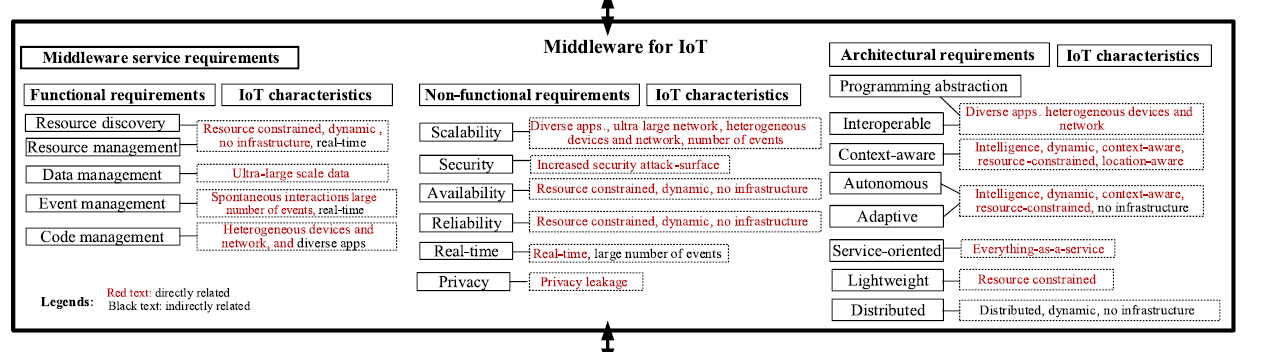
\includegraphics[scale=0.5]{images/requisitos}
%\caption{Requisitos de un middleware IoT.}\label{L105}
%\end{figure}









\chapter{IoT}
La primera vez que se propuso el concepto del Internet de las Cosas fue en 1999 por Kevin Ashton, en el Auto-ID Center del MIT, donde se presentó un sistema de sensores e identificadores de radiofrecuencia (RFID)\\
El nombre de Internet de las cosas (Internet of Things (IoT), en inglés) hace hincapié en la interconexión digital de objetos cotidianos con internet.\\
Un frigorífico que avise de la fecha de caducidad de los alimentos, unas zapatillas de deporte que registren en la nube las estadísticas de la velocidad y distancia a la que corres, un inodoro que analice su orina para que recomiende una dieta u otra, en definitiva, que cualquier cosa u objeto tenga conexión a Internet. \\
Según la empresa Gartner (//////link/////), en 2020 habrá en el mundo unos 26 mil millones de dispositivos con un sistema de conexión al internet de las cosas. Los mencionados objetos se valen por un sistema embebido que permite dotar de inteligencia al objeto conectado, ayudándose de sensores para captar información; esta es otra de las características de IoT, el denominado Big Data: datos, datos y más datos.
IoT puede controlar desde aplicaciones domésticas como las mencionadas anteriormente, a aplicaciones profesionales. Un cultivo en el que cada planta tenga su propio sensor y el agricultor sea capaz en todo momento de recibir información sobre ellas conociendo cómo crecen y si existen problemas en algunas de ellas. \\
El coste que podría tener monitorizar el sistema anterior en el que cada planta tenga un sensor enviando información a ciertos nodos para su procesamiento, podría ser elevado. Por ello se buscan hardware de bajo coste. El uso de sistemas de menor procesamiento hace que se busque nuevas tecnologías o, como mínimo, complementarias a las que existen. Las tecnologías existentes para Internet requieren de hardware con procesamiento elevado. No tiene ningún sentido enviar la información captada por un sensor de humedad (en el que la información recibida es ínfima) mediante HTTP.\\
\begin{figure}[H]
\centering
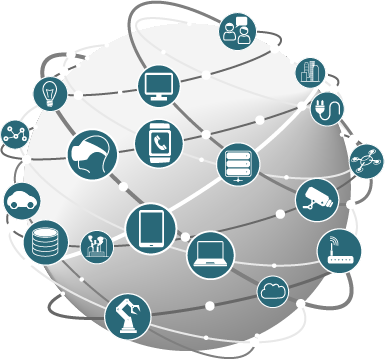
\includegraphics[scale=0.4]{images/iot}
\caption{Internet de las cosas.}\label{L105}
\end{figure}
\section{Barreras en el crecimiento de IoT}
Existen algunos inconvenientes que impiden el avance de IoT. Uno de ellos es el problema de direccionamiento, bien es cierto que ya existe una propuesta firme para cambiar a IPV6. Otro de los principales problemas que impiden el crecimiento de IoT es la seguridad y privacidad. El hecho de compartir información privada en la nube nos hace mucho más vulnerables a los ataques por parte de hackers. Existen casos preocupantes que hacen que la interconexión de todo con todo aún tenga que esperar. \\En 2013, Hugo Teso, un experto en seguridad, demostró, en una maqueta, que era posible tomar el control de un avión desde un dispositivo Android (entre otras cosas), haciéndose valer de información compartida por los aviones para determinar su posición. \\En 2015 un grupo de investigadores descubrió que era relativamente sencillo manipular remotamente la aceleración y el sistema de frenado en los coches autónomos. Ejemplos que nos hacen pensar en la importancia de un sistema de seguridad en IoT y por qué aún no ha dado ese paso definitivo para su expansión. Estos problemas será cuestión de tiempo que se solucionen para que IoT acabe siendo una realidad.
\section{Impacto social}
El internet de las cosas podría cambiar, de hecho lo está haciendo, la vida tal y como la conocemos hoy en día, pues el hecho de que cualquier objeto pueda ser monitoreado nos ayudaría a administrar mejor los recursos. 

\section{Conclusiones}
El IoT se presenta como un nuevo paradigma que parece predestinado a cambiar por completo el escenario socioeconómico tal y como hoy lo conocemos. Estas nuevas tecnologías están permitiendo la obtención de mayores cantidades de información e incluso la obtención de datos sobre elementos de los que antes ni tan siquiera se podía pensar que fuera posible o sobre los que se pudiera influir.\\
Aún con el gran abanico de posibilidades que se abre gracias a la utilización de estas nuevas tecnologías, este nuevo paradigma no se encuentra exento de problemas. Uno de ellos, sino el más
grave, lo constituye su seguridad, en sus múltiples vertientes. Así, según los expertos, la seguridad es un asunto de especial trascendencia, ya que la mayoría de las medidas de seguridad tradicionales no pueden aplicarse al IoT debido principalmente a las restricciones y/o características que comporta su diseño: bajo procesamiento, entornos propensos a ataques malintencionados...\\
Por ello, cuando se superen estos problemas, en los que ya grandes empresas están investigando, IoT dejará de ser usado para entornos en concreto a ser una realidad en nuestras vidas.
\chapter{Middleware en IoT}
\section{Introducción}
Como se ha visto, la esencia de IoT es conectar y comunicar cualquier cosa sobre internet. Conseguir interconectar millones de dispositivos diferentes, trabajando a niveles de red diferentes y generando una gran cantidad de eventos no es una tarea sencilla. Un middleware IoT facilita la integración entre la comunicación de los dispositivos, además de soportar una interoperabilidad dentro de los diferentes servicios y aplicaciones.\\El desarrollo de middleware en IoT es un área activa de investigación. Las líneas de investigación en middleware han ido por las redes de sensores inalámbricas (WSN) /////surveys////, por las comunicaciones máquina a máquina (M2M)////surveys//// o también por etiquetas de identificación de radio frecuencia (RFID) ///surveys///, componentes esenciales en el IoT. En este trabajo se hablará de algunos middleware IoT y finalmente qué middleware es el elegido para su análisis.

\section{CoAP}
CoAP es un protocolo-middleware que trabaja en el dominio de las redes de sensores (WSN) y comunicación M2M. Estas redes requieren de protocolos de transmisión de datos con un ancho de banda reducido y con un consumo muy bajo de energía. CoAP se ha diseñado como una "traducción" sencilla de HTTP para simplificar la integración con la web con requisitos especiales como baja carga, bajo consumo o simplicidad. CoAP implementa el modelo REST de HTTP funcionando sobre UDP y con mecanismos de seguridad específicos para ser usados en este tipo de redes. \\
CoAP es muy usado en IoT, permite descubrimiento de recursos, seguridad, soporte IPv6. En definitiva, un protocolo moderno y con muchos beneficios.
\section{UbiROAD}
UbiROAD es un middleware inteligente conocedor del contexto, esto es, capaz de decidir por él mismo ofreciendo al usuario los servicios necesarios. Se usa en vehículos para el control de tráfico inteligente. 

\section{Agilla}
Agilla\cite{agilla} es un middleware basado en agente diseñado para aplicaciones auto-adaptables en redes de sensores. Las redes de sensores están expuestas a un mundo dinámico, muchas de sus aplicaciones tienen que adaptarse a los cambios en el ambiente. Por ejemplo, una red WSN usada por un robot, tiene que adaptarse a los cambios del robot. En definitiva, se necesitan middleware y nuevos modelos de programación para soportar la auto-adaptabilidad de las redes de sensores. Para tal fin, se desarrolló Agilla\\
La estructura de Agilla está basada en agentes. Un agente no es más que un nodo dotado de inteligencia. Un agente puede clonarse desde un nodo a otro manteniendo su estado y así poder coordinar con otros agentes. La estructura de Agilla se muestra en la figura \ref{agilla}
\begin{figure}[H]
\centering
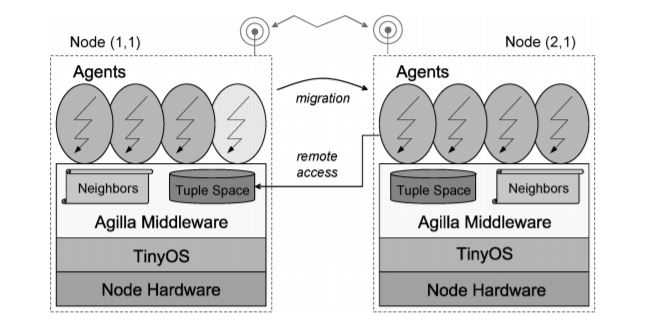
\includegraphics[scale=0.5]{images/agilla}
\caption{Modelo Agilla.}\label{agilla}
\end{figure}
Agilla funciona sobre TinyOS, un sistema operativo para WSN. Un tuplespace es una memoria compartida usada por los agentes para clonarse.
\section{TinySOA}
TinySOA es un middleware usado en redes de sensores. Proporciona un conjunto de servicios Web que facilita el envío y recepción de información por parte de los sensores. La arquitectura se puede ver en la figura \ref{tinysoa}. Está formado por cuatro partes principales: Nodos,gateway,registro y servidor. \\
El nodo reúne toda la información de un nodo sensor. Tiene algunos servicios como el descubrimiento de recursos o la comunicación con el gateway. El gateway en las redes WSN, tiene la función de conectar la red WSN con la red externa, es decir con Internet. Entre otras funcionalidades, usa la información del nodo sensor para registrarlo en el servicio de registro.  Una vez registrados, el gateway se subscribe a los servicios proporcionados por el sensor. El servidor es otra de las partes principales de este middleware, y su función es usar el servicio de registro para establecer un servicio web
\begin{figure}[H]
\centering
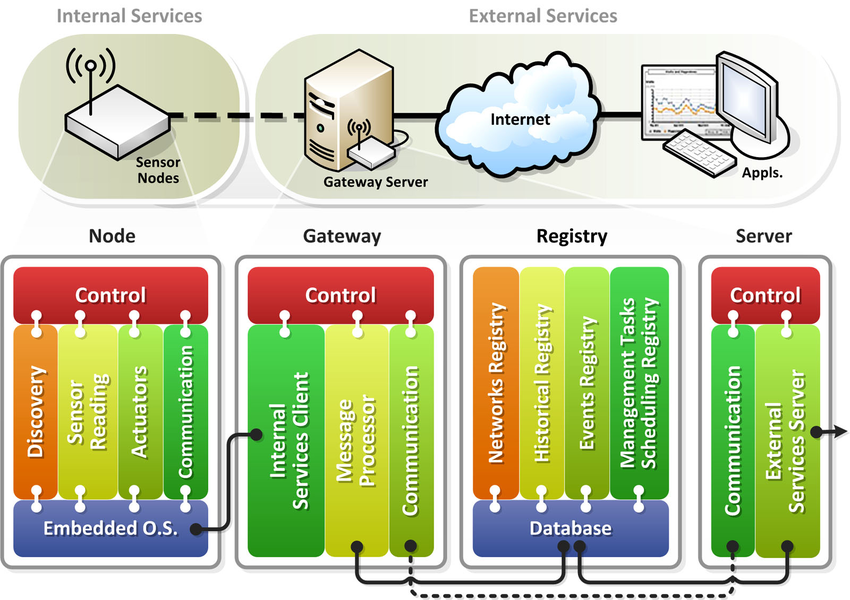
\includegraphics[scale=0.3]{images/tinysoa}
\caption{Arquitectura de TinySOA.}\label{tinysoa}
\end{figure}
\section{MQTT}
El Transporte de telemetría de cola de mensajes (MQTT) es un protocolo de código abierto que se desarrolló y optimizó para dispositivos restringidos y redes de bajo ancho de banda, alta latencia o poco confiables. Es un transporte de mensajería de publicación/suscripción que es extremadamente ligero e ideal para conectar dispositivos pequeños a redes con ancho de banda mínimo. MQTT es eficiente en términos de ancho de banda, independiente de los datos y tiene reconocimiento de sesión continua, porque usa TCP. Tiene la finalidad de minimizar los requerimientos de recursos del dispositivo y, a la vez, tratar de asegurar la confiabilidad y cierto grado de seguridad de entrega con calidad del servicio.

\section{Conclusión}
Con la cantidad de dispositivos existentes y diferentes entre ellos, conectarlos sobre internet es una tarea complicada. Por ello, es necesario un software que facilite la interconexión entre ellos, es aquí donde entra en juego el uso de un middleware. Tras presentar algunos de ellos, se ha optado por elegir MQTT como middleware para ser analizado en mayor profundidad y, en caso de éxito, ser usado en el escenario que planteamos.
\chapter{MQTT}
\section{Introducción}
MQTT (Message Queue Telemetry Transport) es un protocolo usado para la comunicación M2M (Machine to machine) en el internet de las cosas. Fue creado por IBM en 1999. Está orientado a las redes de dispositivos pequeños, como sensores, debido a que consume muy poco ancho de banda además de que no requiere de mucho software para implementar un cliente, lo cual es perfecto para dispositivos como Arduino. MQTT se ha convertido en un protocolo muy usado en IoT, aunque también es ideal para aplicaciones móviles por su envío eficiente. Un ejemplo de uso es Facebook Messenger para iPhone y Android.\\
Se basa en el estandar publish/subscribe usado sobre TCP/IP. Esta comunicación publish/subscribe hace uso de un "broker" o servidor centralizado para la gestión de los paquetes.

\begin{figure}[h!]
\centering
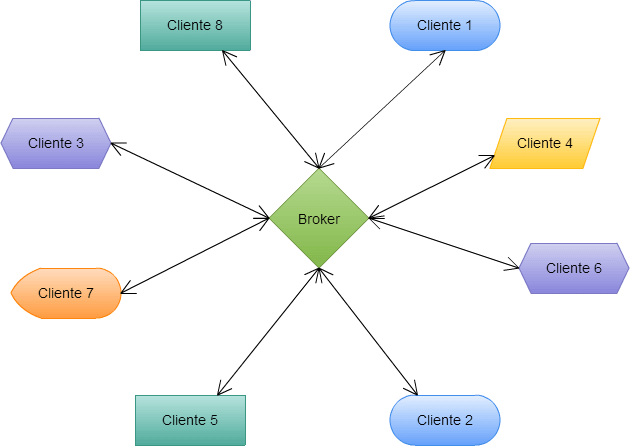
\includegraphics[scale=0.3]{images/topologia.png}
\caption{Topología MQTT.}\label{L401}
\end{figure}
\newpage
%\vspace*{1.8cm}
La comunicación se basa en "topics" (temas) que el cliente que publica el mensaje envía y los nodos que desean recibirlo deben subscribirse a él. Un topic se representa mediante una cadena de caracteres separada por "/". De esta forma se pueden crear jerarquías como se puede ver en la figura \ref{L402} \
\begin{figure}[h!]
\centering
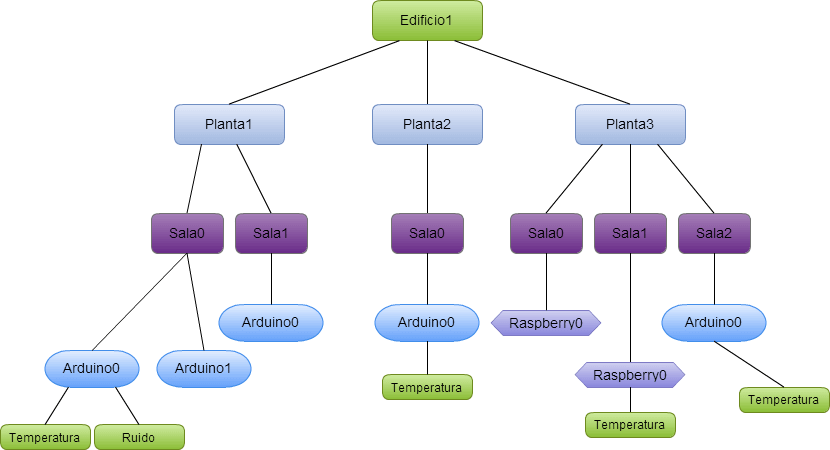
\includegraphics[scale=0.3]{images/jerarquia.png}
\caption{Jerarquía Topics.}\label{L402}
\end{figure}
\section{Protocolo}
MQTT funciona sobre TCP y, como cualquier protocolo, tiene un esquema definido para el envío y recepción de paquetes. El código y tipo de paquete se definen en la siguiente tabla.
\begin{table}[H]
\centering
\begin{tabular}{lcl}
\rowcolor[HTML]{00D2CB} 
Paquete     & Enumeración & Descripción                                        \\
Reservado   & 0           & Reservado                                          \\
CONNECT     & 1           & Cliente solicita conectarse al servidor            \\
CONNACK     & 2           & Confirmación del mensaje CONNECT                   \\
PUBLISH     & 3           & Mensaje PUBLISH                                    \\
PUBACK      & 4           & Confirmación del paquete PUBLISH                   \\
PUBREC      & 5           & PUBLISH recibido ()                                \\
PUBREL      & 6           & PUBLISH release ()                                 \\
PUBCOMP     & 7           & Publish completado                                 \\
SUBSCRIBE   & 8           & Petición del cliente para subscribirse a un tópico \\
SUBACK      & B           & Confirmación del paquete SUBSCRIBE                 \\
UNSUBSCRIBE & 10          & Petición del cliente para desuscribirse            \\
UNSUBACK    & 11          & Confirmación de UNSUBSCRIBE                        \\
PINGREQ     & 12          & PING                                               \\
PINGRESP    & 13          & Respuesta PING                                     \\
DISCONNECT  & 14          & Cliente se va a desconectar                        \\
Reservado   & 15          & Reservado                                         
\end{tabular}
\caption{Enumeración de paquetes}
\label{table:package}
\end{table}
Una vez realizada la conexión a nivel de red entre cliente y broker mediante el envío de los paquetes CONNECT y CONNACK, el cliente se subscribe a un topic. El flujo de datos es el que se muestra en la figura \ref{L403}. El cliente envía un paquete "SUBSCRIBE" con el que el cliente le dice a qué topics quiere subscribirse. Cada suscripción será confirmada por el broker mediante el envío de un paquete "SUBPACK". El broker envía en el paquete un código de respuesta por cada topic al que el cliente se ha suscrito, en el mismo orden que el cliente lo envió. El código de respuestas se puede ver en la tabla \ref{table:return_code}. Una vez recibida la confirmación, el cliente puede empezar a enviar mensajes.
\begin{figure}[H]
\centering
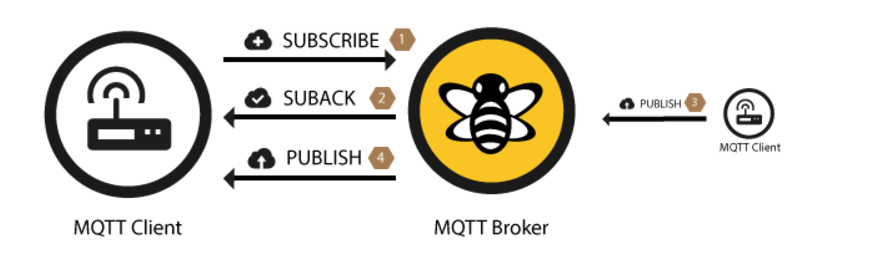
\includegraphics[scale=0.5]{images/flujo_tipico.png}
\caption{Envío de paquetes en MQTT.}\label{L403}
\end{figure}
\begin{table}[htbp]
\begin{center}
\begin{tabular}{|l|l|}
\hline
Return Code & Return Code response \\
\hline \hline
0 & Success – Maximum QoS 0 \\ \hline
1 & Success – Maximum QoS 1 \\ \hline
2 & Success – Maximum QoS 2 \\ \hline
128 & Failure
\end{tabular}
\caption{Código de respuesta}
\label{table:return_code}
\end{center}
\end{table}


\begin{figure}[H]
\centering
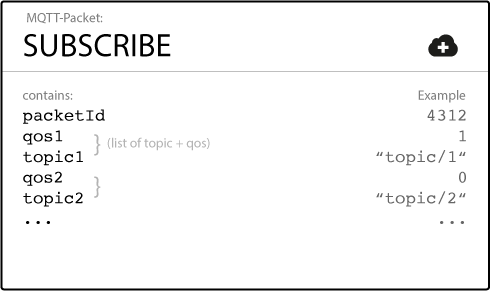
\includegraphics[scale=0.3]{images/subscribe_packet.png}
\caption{Paquete SUBSCRIBE.}\label{L404}
\end{figure}
\begin{figure}[H]
\centering
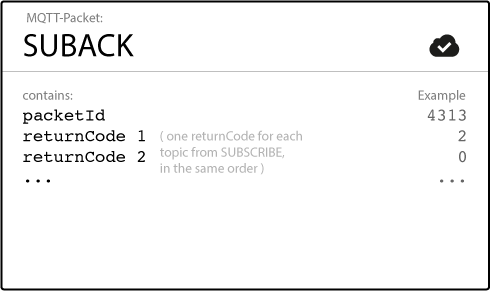
\includegraphics[scale=0.3]{images/suback_packet.png}
\caption{Paquete SUBACK.}\label{L405}
\end{figure}

Por otro lado, si el cliente quiere desuscribirse a un topic deberá enviar un paquete "UNSUBSCRIBE" y esperar la confirmación por parte del broker mediante el paquete "UNSUBACK"
\begin{figure}[H]
\centering
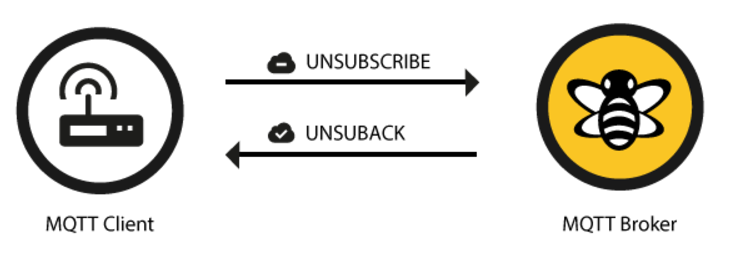
\includegraphics[scale=0.5]{images/flujo_desuscribir.png}
\caption{Envío de paquetes para desuscribirse de un topic.}\label{L406}
\end{figure}
\begin{figure}[H]
\centering
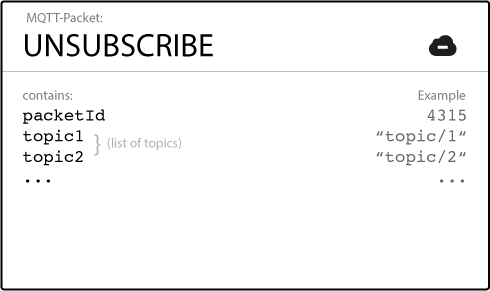
\includegraphics[scale=0.3]{images/unsubscribe_packet.png}
\caption{Paquete UNSUBSCRIBE.}\label{L407}
\end{figure}
\begin{figure}[H]
\centering
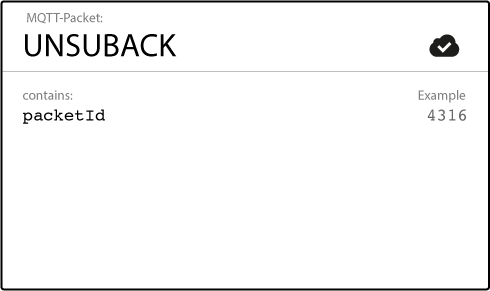
\includegraphics[scale=0.3]{images/unsuback_packet.png}
\caption{Paquete UNSUBACK.}\label{L408}
\end{figure}
\subsection*{Brokers}
Es el servidor de MQTT. El broker recibe los mensajes por parte de los clientes y se encarga de procesar y enviar el mensaje a los subscriptores de ese topic. La gestión de la red es otra de las funcionalidades del broker. Los clientes envían periódicamente un paquete (PINGREQ) y esperan la respuesta del broker (PINGRESP) para mantener activo el canal.\\
Existen varias empresas como HiveMQ \cite{hive}\cite{hive_doc} que comercializan un broker MQTT diseñado por ellos mismos. Otro broker comercial es CloudMQTT \cite{cloud_mqtt}, propiedad de Amazon.

En este documento se trabajará con el broker Mosquitto \cite{mosqtt}, el cual es de código abierto y es uno de los más usados y completos que existen.

En la siguiente tabla se muestra una comparación entre alguno de los brokers más usados.
\begin{table}[H]
\centering

\begin{tabular}{lcccccccc}
\cellcolor[HTML]{00D2CB}Broker    & \cellcolor[HTML]{00D2CB}QoS0 & \cellcolor[HTML]{00D2CB}QoS1 & \cellcolor[HTML]{00D2CB}QoS2 & \cellcolor[HTML]{00D2CB}Autenticación & \cellcolor[HTML]{00D2CB}Bridge & \cellcolor[HTML]{00D2CB}SSL & \cellcolor[HTML]{00D2CB}Clustering & \cellcolor[HTML]{00D2CB}WebSocket \\
Mosquitto & \cmark                       & \cmark                       & \cmark                       & \cmark                                & \cmark                         & \cmark                      & \xmark                             & \cmark                                \\
Mosca     & \cmark                       & \cmark                       & \xmark                       & \cmark                                & \xmark                         & \cmark                      & \xmark                             & \cmark                                \\
HiveMQ    & \cmark                       & \cmark                       & \cmark                       & \cmark                                & \cmark                         & \cmark                      & \cmark                             & \cmark                                \\
ActiveMQ  & \cmark                       & \cmark                       & \cmark                       & \cmark                                & \xmark                         & \cmark                      & \cmark                             & \cmark                                \\
VerneMQ   & \cmark                       & \cmark                       & \cmark                       & \cmark                                & \cmark                         & \cmark                      & \cmark                             & \cmark                                \\
JoramMQ   & \cmark                       & \cmark                       & \cmark                       & \cmark                                & \cmark                         & \cmark                      & \cmark                             & \cmark                               
\end{tabular}
\caption{Comparación entre brokers MQTT}
\label{broker_comparasion}
\end{table}
MQTT Websocket surge para usar MQTT sobre HTTPy poder usar un cliente MQTT en un navegador. Esto es útil cuando se quiera enviar los datos a dispositivos situados en el exterior de la red, como por ejemplo servidores. Estos dispositivos tendrán que tener un nivel de procesamiento más elevado que los de la red interna, pues HTTP necesita de dispositivos más potentes. 
\begin{figure}[H]
\centering
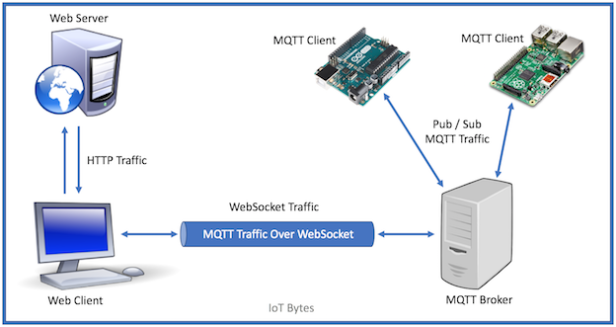
\includegraphics[scale=0.7]{images/mqtt_over_websockets}
\caption{MQTT sobre WebSockets}\label{L409}
\end{figure}
\subsection*{Clientes}
Se encargan de enviar al broker la información recibida, normalmente por parte de sensores. Los clientes también reciben mensajes de los topics subscritos.
Al igual que los brokers, hay muchos tipos de clientes MQTT. El cliente Open-Source más usado es Eclipse Paho Java Client \cite{paho}
\section{MQTT-SN}
\subsection{Redes de sensores inalámbricas}
Las redes de sensores o Wireless Sensor Networks (WSN) en inglés, se han incrementado en los últimos años. Estas redes tienen diferentes aplicaciones, como puede ser la vigilancia y seguridadd, medicina, domótica o aplicaciones militares. Una red de sensores está formada por sensores y gateway para conectar con una red de datos. En estas redes es importante la comunicación de forma inalambrica entre sensores, puesto que el número de nodos (sensores, actuadores...) es muy grande, y una infraestructura cableada tendría un coste muy elevado. Las características de estas redes son:
\begin{itemize}
\item[•]Tolerancia a fallos\\
\item[•]Coste\\
\item[•]Ausencia de infraestructura de red\\
\item[•]Bajo consumo
\end{itemize} 
A diferencia de las redes convencionales, los nodos no tienen conocimiento de la topología de la red, por lo que el enrutamiento cambia con respecto a éstas. Aquí es el nodo el que se informa de los nuevos nodos a su alcance y de la manera de encaminarse hacia ellos. En la figura \ref{L411} se puede ver la estructura de una red de este tipo.
\begin{figure}[H]
\centering
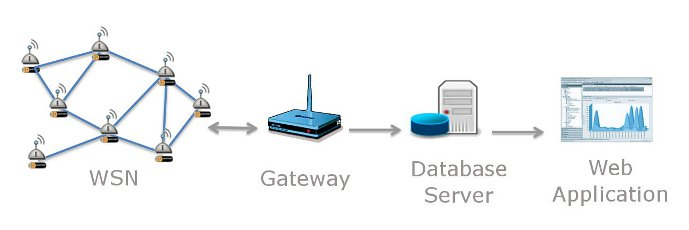
\includegraphics[scale=0.5]{images/wsn}
\caption{Multi level}\label{L411}
\end{figure}
 
\subsection{MQTT-SN}
MQTT es un protocolo usado sobre redes donde el ancho de banda sea limitado, sin embargo MQTT requiere del protocolo TCP/IP, útil para redes con dispositivos de aceptable procesamiento, puesto que ofrece una entrega correcta de los paquetes pero es demasiado complejo como para ser usado en redes de sensores, en las que los dispositivos son de poca memoria y de bajo procesamiento.\\
Es por ello donde surge MQTT-SN, un protocolo pub/sub específico para redes de sensores. 
\subsection{Arquitectura MQTT-SN}
La arquitectura MQTT-SN se muestra en la figura \ref{L412}
\begin{figure}[H]
\centering
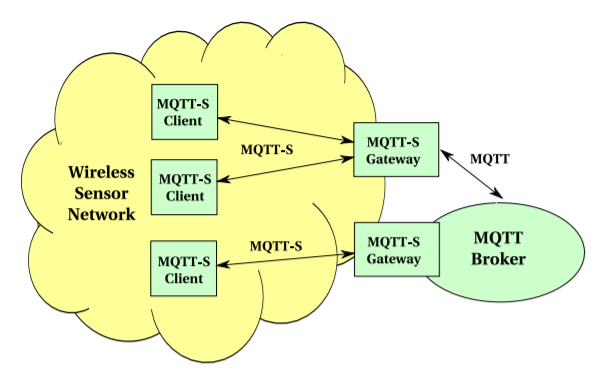
\includegraphics[scale=0.5]{images/mqttsn}
\caption{Arquitectura MQTT-SN}\label{L412}
\end{figure}
Hay 2 componentes: MQTT-SN clientes y MQTT-SN gateways. Los MQTT-SN clientes son los nodos en la red WSN. La comunicación entre clientes se hace a través del Gateway mediante el protocolo MQTT-SN. Los clientes realizan la comunicación pub/sub con un broker, localizado en una red tradicional, a través del Gateway. La comunicación entre el broker y el MQTT-Gateway se hace mediante el protocolo MQTT.
\subsection{Funcionamiento}  
\subsection{MQTT vs MQTT-SN}
MQTT-SN se diferencia en MQTT en varios aspectos. A nivel de red, no funciona sobre TCP pero necesita de Gateways para su funcionamiento.
MQTT-SN soporta ID de topics en lugar de nombres, siempre es menos costoso enviar el ID en cada mensaje que no el nombre completo ("home/livingroom/socket2/meter"). \\
El descubrimiento es una de las mayores ventajas de MQTT-SN. Los clientes no necesitan saber la dirección IP o DNS del broker. El anunciamiento ayudará a descubrir los nodos. Los gateways de la red envían paquetes cada cierto periodo de tiempo advirtiendo de su presencia. Los clientes tienen que guardar una lista de los gateways activos junto con su dirección de red. Esta lista se forma a partir de los paquetes ADVERTISE y GWINFO enviados por los gateways. El cliente puede usar esta lista para conocer la disponibilidad de los gateways. Por ejemplo, si no recibe el mensaje ADVERTISE durante un tiempo determinado puede considerar que está caído y actualizar la lista. Conociendo la dirección de red del gateway el cliente puede conectarse mediante el envío de paquetes, como se hace en MQTT, aunque en este caso el paquete CONNECT, se divide en varios paquetes.\\
%Se puede integrar MQTT y MQTT-SN preparando el gateway para establecer una comunicación con un broker MQTT. Esto es útil cuando exista una red de sensores a bajo nivel pero se quiera un mayor procesamiento a niveles más altos. También es útil si se buscan los requisitos que ofrece MQTT-SN como pueda ser el descubrimiento de recursos.
%\begin{figure}[h!]
%\centering
%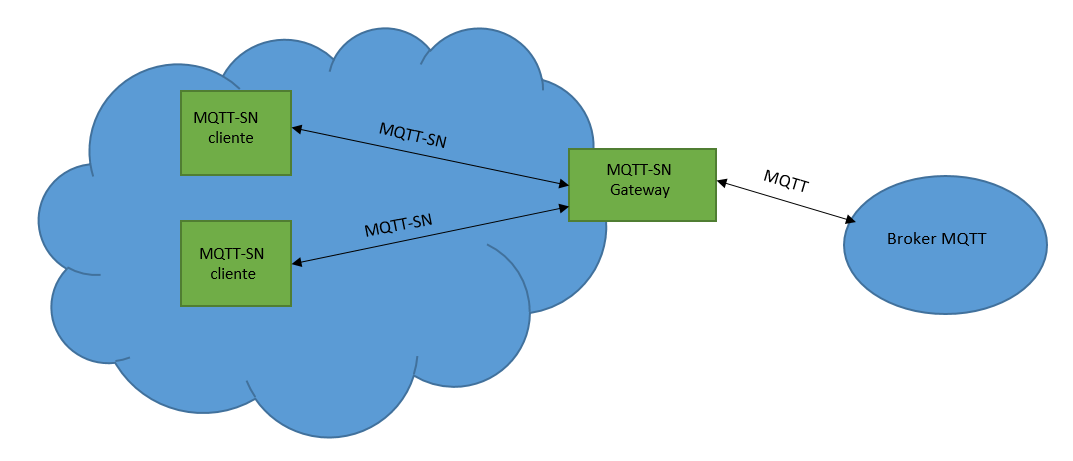
\includegraphics[scale=0.4]{images/mqtt_mqttsn}
%\caption{Arquitectura MQTT-SN.}\label{L4015}
%\end{figure}


\section{Requisitos}
MQTT como middleware IoT, necesita cumplir una serie de requisitos. En el escenario que se plantea hay algunos que no son indispensables y otro que sí lo son, como pueda ser la seguridad. Aquí se definen algunos de los requisitos.
\subsection{Requisitos funcionales}
\subsubsection*{Descubrimiento de recursos}
En MQTT no hay un mecanismo para el descubrimiento de recursos. El cliente se tiene que conectar al broker para su comunicación. Con MQTT-SN, una extensión de MQTT para redes de sensores, sí que hay un mecanismo de descubrimiento de nuevos dispositivos.
\subsubsection*{Control de recursos}
MQTT realiza un control básico a nivel de red. Si el broker percibe (mediante el temporizador "keep alive" en el envío de PINGREQ) una desconexión inesperada del cliente, el broker publica un mensaje "Last Will and Testament" (LWT) a todos los subscriptores de ese topic. Los clientes cuando se conectan al broker, tienen la opción de definir este mensaje y  pedir al broker que lo almacene.\\
Existen herramientas que realizan un control y monitorización más avanzados como MQTTSpy. MQTTSpy se ejecuta sobre Java y se pueden obtener estadísticas sobre los tópicos.
\subsubsection*{Control de datos}
MQTT proporciona un control de datos como son el almacenamiento o el filtrado. De todo ello se encarga el broker. El broker puede almacenar los paquetes de un tópico mientras el cliente, subscrito a dicho tópico, esté offline. El broker también puede aplicar un filtrado en los tópicos, para que se aplique a un nivel o a todos los niveles de ese tópico:
\begin{itemize}
\item[•]\textbf{Single level : +} \\
\begin{figure}[h!]
\centering
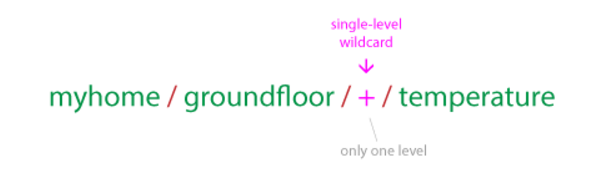
\includegraphics[scale=0.5]{images/figure4}
\caption{Single level}\label{L409}
\end{figure}
Para que el mensaje llegue a un cliente, éste debe de estar subscrito a un tópico en el que solamente cambie el nivel indicado por el signo +. En este ejemplo, el mensaje destinado a \textbf{myhome/groundfloor/livingroom/temperature} o \textbf{myhome/groundfloor/kitchen/temperature} llegaría al cliente. Sin embargo, un mensaje destinado a \textbf{myhome/groundfloor/kitchen/brightness} o \textbf{myhome/firstfloor/kitchen/temperature} no llegaría al cliente.
\item[•]\textbf{Multi level: \#}\\
\begin{figure}[h!]
\centering
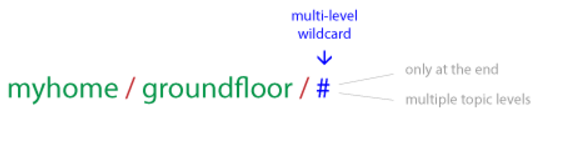
\includegraphics[scale=0.5]{images/figure5}
\caption{Multi level}\label{L410}
\end{figure}
En este caso, llegaría a cualquier cliente que esté subscrito a partir de ese nivel.\\
Los tópicos que empiecen por el símbolo \$ están reservados para las estadísticas internas del broker MQTT. Un ejemplo puede ser:
\begin{itemize}
\item[•]\$SYS/broker/clients/connected
\item[•]\$SYS/broker/clients/disconnected
\item[•]\$SYS/broker/clients/total
\item[•]\$SYS/broker/messages/sent
\end{itemize}
\end{itemize}
\subsubsection*{Control de eventos}

\subsubsection*{Control de código}

\subsection{Requisitos no funcionales}
\subsubsection*{Escalabilidad}
MQTT tiene, en general, una alta escalabilidad, que va a depender en gran medida de la calidad de los nodos y de la topología que se use. La existencia de uno o más brokers dota al sistema de gran escalabilidad ya que la solución puede crecer solo con aumentar recursos en un único elemento.
Para añadir un nuevo cliente, tan solo es necesario suscribirse a un topic.
\begin{figure}[h!]
\centering
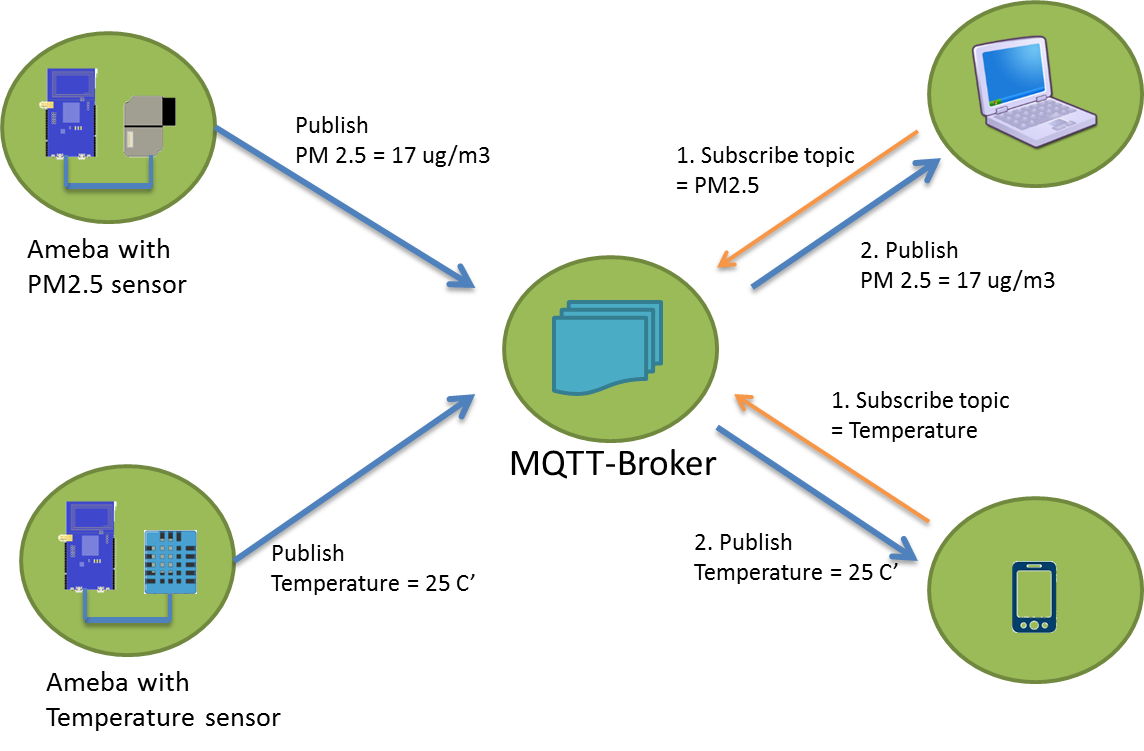
\includegraphics[scale=0.3]{images/figure3.png}
\caption{Escalabilidad MQTT}\label{L403}
\end{figure}
\subsubsection*{Seguridad y privacidad}
La seguridad es vital en un entorno IoT y para ello MQTT usa TLS junto con una autenticación de usuario/contraseña. Usa una autenticación usuario/contraseña a nivel de aplicación para establecer la conexión entre cliente y broker. Si TLS se resuelve correctamente, entra en juego dicha autenticación. Además, también existen políticas de autorización para denegar un determinado topic o para permitir una operación
\begin{figure}[h!]
\centering
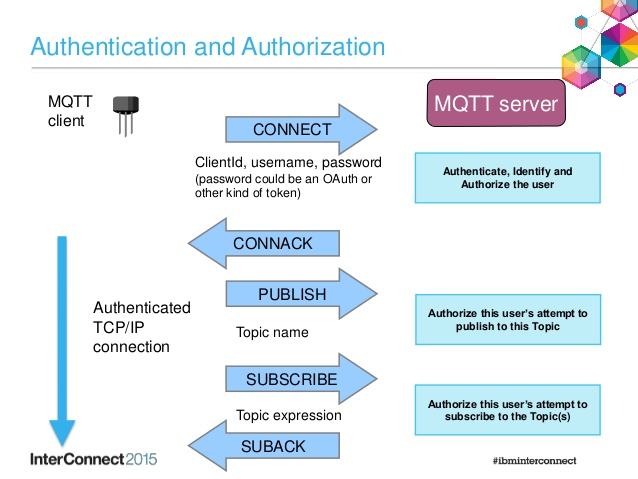
\includegraphics[scale=0.3]{images/mqtt_ssl}
\caption{Autenticación MQTT}\label{L404}
\end{figure}
\subsubsection*{Disponibilidad}
Debido a su arquitectura ///"brokerizada"///, los sistemas MQTT tiene un único punto de fallo: el broker. La disponibilidad del sistema es baja al basarse únicamente en la disponibilidad del broker. \\
Con herramientas como balanceadores de carga, o el uso de los brokers en modo “bridge” se puede conseguir una buena disponibilidad. La disponibilidad permitirá poder seguir usando la red en caso de fallo en alguno de sus nodos. 

Con el denominado MQTT clustering se incrementa la disponibilidad. MQTT clustering consiste en usar varios brokers (cluster) MQTT como si de uno solo se tratase. Esto se consigue usando brokers en diferentes dispositivos físicos y conectándolos a nivel de red. A vista del cliente MQTT, estos brokers se comportan como un único broker. Se usan balanceadores de carga para tener un único punto de entrada y mejorar así el consumo en la red. En la siguiente imagen se puede ver un ejemplo de clustering con el broker comercial HiveMQ.
\begin{figure}[H]
\centering
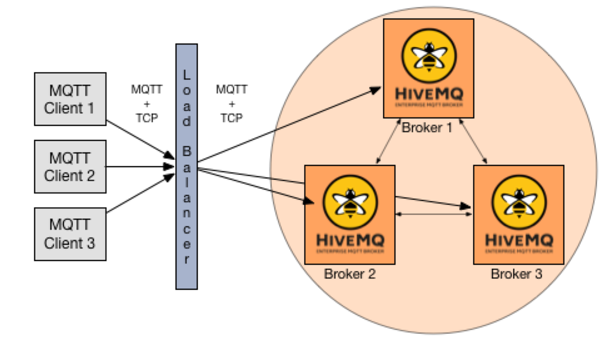
\includegraphics[scale=0.3]{images/mqtt_clustering.png}
\caption{MQTT Clustering.}\label{L406}
\end{figure}

Mosquitto no tiene esta característica pero se podría mejorar la disponibilidad utilizando el broker en modo "bridge". Con el modo "bridge" configurado, se puede enviar información entre los brokers y así eliminar un único punto de fallo, mejorando la disponibilidad. 
\begin{figure}[H]
\centering
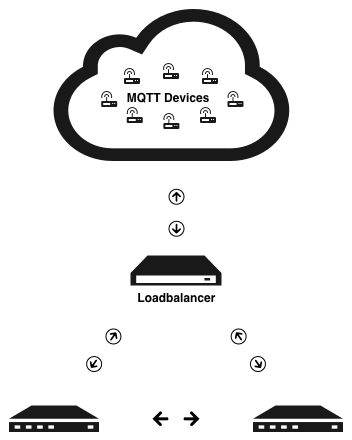
\includegraphics[scale=0.3]{images/mqtt_availability.png}
\caption{MQTT en modo bridge.}\label{L405}
\end{figure}
\subsubsection*{Confiabilidad}
MQTT proporciona 3 grados de QoS para la entrega de los paquetes:
\begin{itemize}
\item[•]\textbf{QoS 0: Como mucho una vez}\\
El mensaje PUBLISH se envía y el broker no manda ningún reconocimiento. El mensaje llega al broker una vez o ninguna y si llega, llegará a los subscriptores una vez o ninguna.
\begin{figure}[h!]
\centering
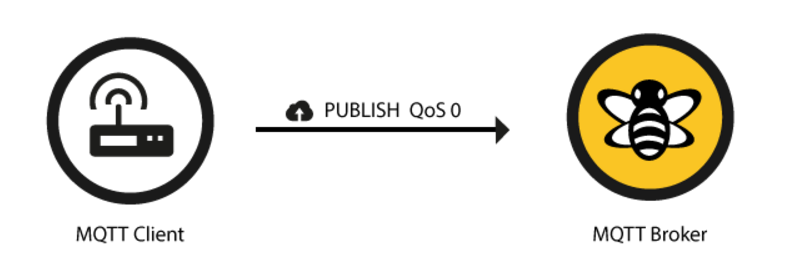
\includegraphics[scale=0.3]{images/qos0}
\caption{QoS 0}\label{L406}
\end{figure}
\item[•]\textbf{QoS 1: Al menos una vez}\\
Este nivel de calidad de servicio asegura que llega al broker al menos una vez. El broker tiene que reconocer la recepción con un paquete PUBACK. Si no recibe un acuse de recibo se vuelve a enviar de nuevo el mensaje PUBLISH con otro identificador distinto hasta que se reciba el reconocimiento. En este nivel no se garantiza que los paquetes no lleguen duplicados.
\begin{figure}[H]
\centering
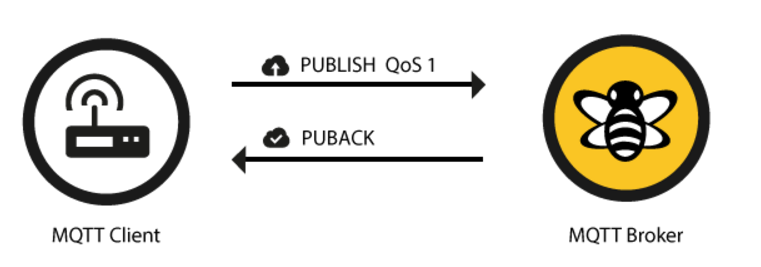
\includegraphics[scale=0.3]{images/qos1}
\caption{QoS 1}\label{L407}
\end{figure}
\item[•] \textbf{QoS 2: Exactamente una vez}\\
Este nivel de calidad asegura que el paquete llega una y solo una vez. Para ello se deben enviar además los paquetes PUBREC y PUBREL.
\begin{figure}[h!]
\centering
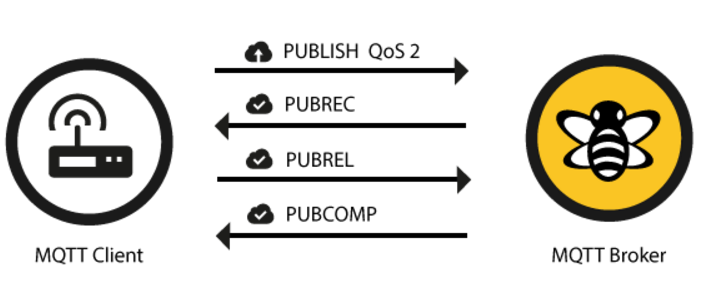
\includegraphics[scale=0.3]{images/qos2}
\caption{QoS 2}\label{L408}
\end{figure}
\end{itemize}
\subsubsection*{Tiempo real}
Si tiempo real lo definimos en microsegundos, MQTT no cumple este requisito ya que una de las principales características de MQTT es que funciona sobre TCP. En el escenario que se plantea, estos microsegundos no son necesarios por lo que no es un requisito indispensable.

\subsubsection*{Fácil de desplegar}
MQTT es un protocolo que destaca por su sencillez
\subsubsection*{Popularidad}
MQTT es un middleware muy usado debido a su consumo y facilidad de uso. Tiene un gran soporte así como empresas que comercializan sus propios brokers añadiéndole mejoras y usándolo en aplicaciones IoT.
\subsection{Requisitos arquitectónicos}
\subsubsection*{Abstracción de la programación}

\subsubsection*{Interoperabilidad}
MQTT es un protocolo heterogéneo en cuanto a dispositivos y tecnologías se refiere. Puede funcionar prácticamente en cualquier dispositivo ya que es un protocolo muy sencillo que requiere poco procesamiento. Puede funcionar en un dispositivo móvil, PC, Raspberry…
\subsubsection*{Autónomo}

\subsubsection*{Distribuido}
Esta característica dependerá del broker a usar, algunos como HiveMQ o JoramMQ, pueden actuar como sistemas distribuidos, en los que se interpreta un cluster de brokers como un único broker.
El broker Open-Source Mosquitto no cumple con este requisito.
\subsubsection*{Orientado a servicio}

\subsubsection*{Ligero}
El bajo consumo de MQTT es una de las claves de su uso extendido en IoT. MQTT está diseñado para trabajar con dispositivos de bajo procesamiento como sensores o dispositivos móviles. Además, el consumo de ancho de banda que realiza en la red es mínimo. 

\subsubsection*{Adaptativo}

\subsection{Documentación}
MQTT es un middleware de código abierto perfectamente
\MYhref{http://docs.oasis-open.org/mqtt/mqtt/v3.1.1/mqtt-v3.1.1.html}{documentado}. Es sencillo de usar y hay una gran cantidad de ejemplos para facilitar su despliegue.\\

 
\section{Cloud Computing}
En IoT se busca un procesamiento en la nube. MQTT nos ofrece el envío de datos y pequeños controles sobre los mismos pero para obtener una solución IoT completa se necesita de servidores y bases de datos. Algunos de los escenarios típicos con MQTT hacen uso de herramientas como Node-RED\cite{nodered} junto con MongoDB\cite{mongo}. MQTT se encargaría del envío de datos (como se ha explicado más arriba) y éstos se enviarían al servidor, donde Node-RED recopilaría esos datos y los almacenaría en MongoDB. Se pueden usar herramientas como Google Chart para analizar los datos y poder llevar un control en tiempo real sobre los mismos. 
\begin{figure}[H]
\centering
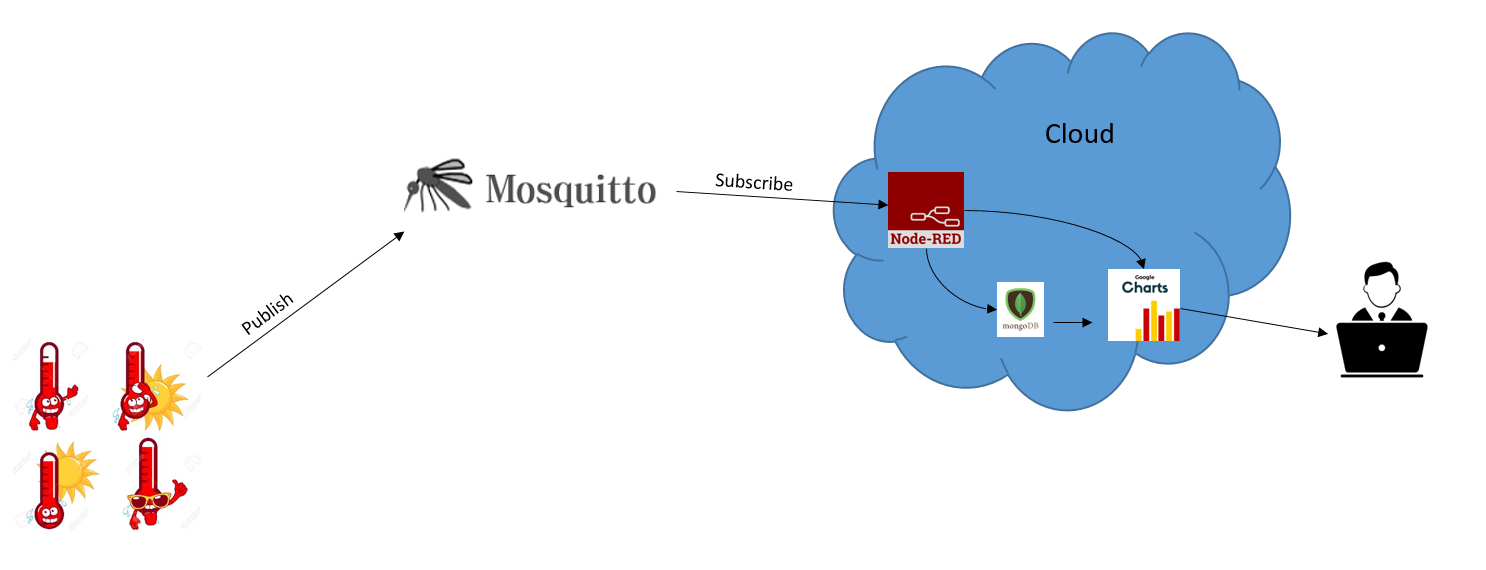
\includegraphics[scale=0.4]{images/cloud_mqtt1}
\caption{Cloud Computing haciendo uso de MQTT}\label{L408}
\end{figure}
\section{Conclusiones}
MQTT como middleware IoT, puede dar solución a múltiples problemas. MQTT cumple con lo que buscamos en cuanto a requisitos se refiere pero no nos ofrece una solución completa. Por ello hemos optado por buscar plataformas-middleware Open-Source que nos ofrezca una solución más completa.Es decir, un middleware que unifique almacenamiento en la nube, procesamiento y análisis de datos...

\chapter{Plataformas IoT}
\section{Introducción}
Hoy en día, se ha incrementado el número de soluciones middleware para IoT que proporciona una interconexión entre los dispositivos y los datos. Estas soluciones middleware se aplican a escenarios en concreto, como el caso de MQTT que se aplica a nivel de transporte para facilitar la comunicación M2M o, el caso de Agilla para redes de sensores en las que se busca un ambiente de auto-adaptación. Es decir, no existe un middleware que ofrezca una solución completa, desde el control de dispositivos  y la recolección de datos hasta el procesamiento y visualización de los mismos. Es aquí donde surge la idea de una plataforma-middleware IoT\cite{platform_gap} que integre esos servicios. Este panorama, como cualquier concepto de IoT, inexistente hace unos años, es complejo y cambiante de manera rápida. Estas plataformas residen en la nube y permiten al usuario reunir los datos de sensores y actuadores y procesarlos, bien para almacenarlos, bien para visualizarlos o bien para analizarlos y extraer información útil de ellos.
\begin{figure}[H]
\centering
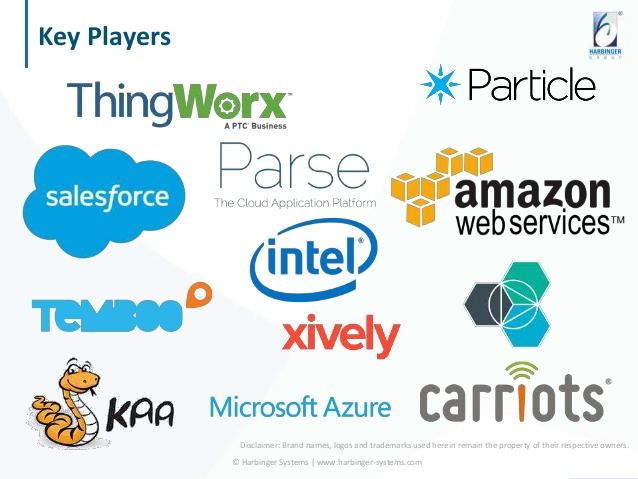
\includegraphics[scale=0.3]{images/platforms_iot}
\caption{Plataformas IoT}\label{platforms_iot}
\end{figure}
\section{Características}
La estructura de IoT se muestra en la figura \ref{stack_iot}, el objetivo de una plataforma IoT es facilitar la integración de esos niveles: conectividad, servicios y nube, aplicaciones y análisis.
\begin{figure}[H]
\centering
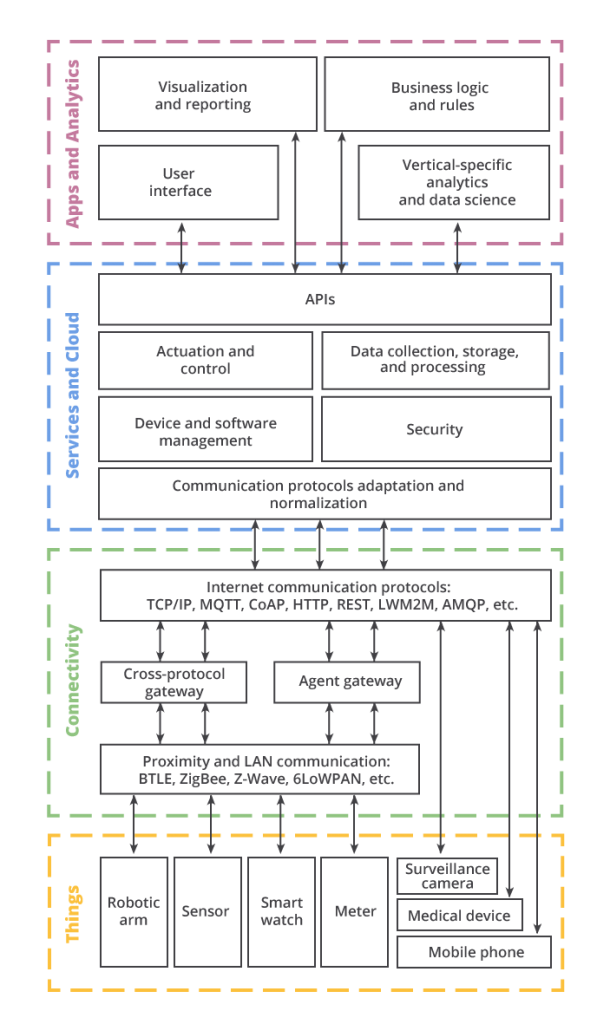
\includegraphics[scale=0.4]{images/iot_stack}
\caption{Pila de tecnologías en IoT}\label{stack_iot}
\end{figure}
Algunas características que poseen las plataformas son:
\subsubsection*{Seguridad y privacidad}
Un criterio fundamental para las plataformas IoT es el uso de mecanismos eficientes de seguridad y privacidad
\subsubsection*{Basada en nube}
Una plataforma IoT es una solución que "vive" en la nube. Pueden ser controladas y accesibles desde cualquier lado.
\subsubsection*{Integración de tecnologías}
La heterogeneidad de diferentes tecnologías es la esencia de las plataformas IoT. Una plataforma ideal, ofrecería un conjunto de protocolos de comunicación donde el usuario elige el protocolo apropiado.
\subsubsection*{Propiedad de los datos}
Esta es una de las preocupaciones de las plataformas IoT, pues en un entorno en el que se envía enormes volúmenes de datos a la nube, es difícil garantizar la propiedad total de los datos. Solo soluciones donde propiedad alamacenan los datos localmente son las que ofrecen una completa privacidad de los datos. El desarrollo de algoritmos y mecanismos que garanticen esta propiedad es una de las tareas pendientes de las plataformas IoT.
\subsubsection*{Análisis de datos}
El análisis de datos es una de las características principales de las plataformas IoT. Una vez subidos los datos a la nube se analizan bien con herramientas propias de la plataforma o bien con herramientas de análisis de datos externas a ella.
\subsection{Plataformas}
Existen cientos de plataformas IoT tanto Open-Source como con licencia comercial. Algunas empresas buscan hacerse un hueco en el mercado IoT con el desarrollo de estas plataformas. 
\begin{itemize}
\item[•]\textbf{Amazon Web Services: }Amazon domina el mercado de la nube. Fueron los primeros en traer el Cloud-Computing allá por el 2004. Su plataforma es extremadamente escalable soportando millones de interacciones entre los dispositivos y el servidor. Usa sus propios servicios para el funcionamiento de la plataforma. 
\item[•]\textbf{IBM Watson: }IBM es otro gigante IT que ha fijado su objetivo en el IoT. Su plataforma busca la facilidad para acceder a sus servicios en la nube. Se puede, entre otros, almacenar datos por un periodo de tiempo definido u obtener información de los dispositivos conectados.  
\item[•]\textbf{Salesforce: } Salesforce es una plataforma impulsada por Thunder, la cual se basa en alta velocidad y tiempo real en las decisiones en la nube.
\end{itemize}


En la siguiente tabla\cite{platform_gap} se muestran las características de algunas plataformas IoT.
\begin{figure}[H]
\centering
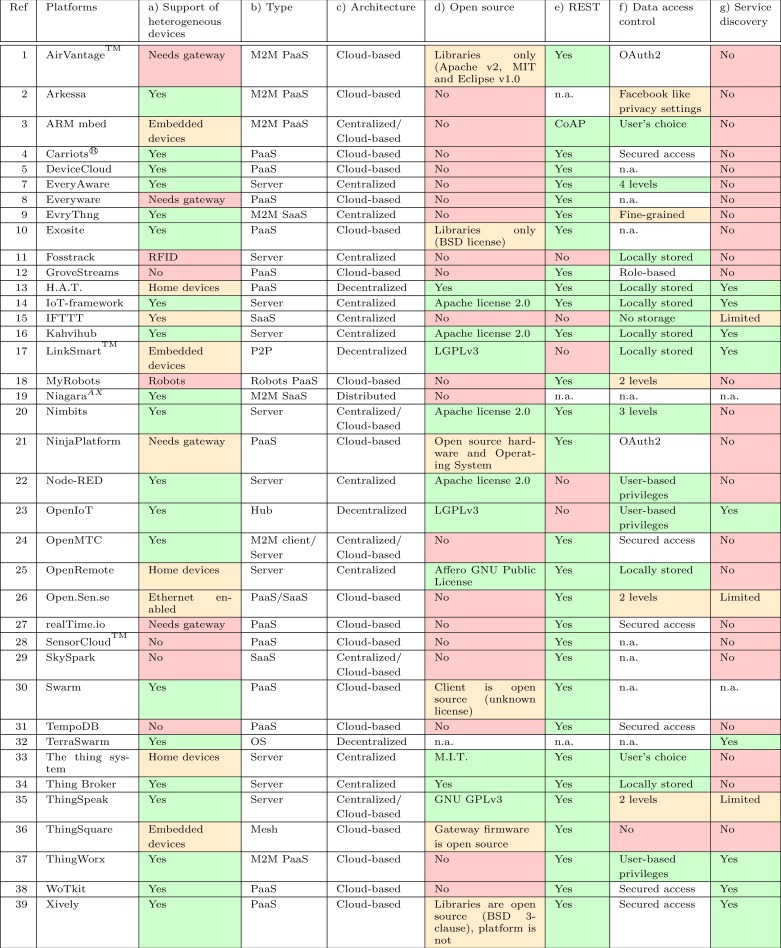
\includegraphics[scale=0.7]{images/platforms}
\caption{Caracterísitcas de algunas plataformas IoT.}\label{L400}
\end{figure}
\section{Conclusiones}
El rápido y cambiante mundo de IoT necesita de plataformas software que ayuden a disminuir la separación existente entre hardware y software, integrando varios servicios como: recolección de datos, seguridad, análisis en tiempo real, en una única plataforma-middleware IoT. En este capítulo se han descrito algunas características de las plataformas IoT. No existe la plataforma perfecta, cada una ofrece ciertos servicios y es el usuario quien tiene que decidir cuál usar. En los siguientes capítulos se analizarán OpenIoT y Kaa como plataformas IoT Open-Source en mayor profundidad. Se elegirá, según nuestro criterio, la más adecuada para desplegar el escenario planteado al inicio de este documento.
\chapter{OpenIoT}
\section{Introducción}
A pesar de la expansión de las aplicaciones IoT en la nube, la ausencia de una semántica que proporcione una interoperabilidad entre las diferentes aplicaciones es una de las principales limitaciones de IoT. Esta ausencia de una unificación se refleja en los diferentes vocabularios y formas para describir las cosas/objetos físicos. No existe un modelo a seguir para integrar todos los servicios, como sí existe en redes IP. \\

OpenIoT\cite{openiot}\cite{openiot_git}\cite{openiot_pdf} surge como un proyecto europeo que busca la unificación de esas soluciones. Se trata de una plataforma de código abierto que proporciona una convergencia entre los diversos sistemas IoT. Mezcla el concepto Cloud-Computing con el concepto de redes de sensores de IoT.\\ 

OpenIoT se basa en SSN como el modelo para la unificación de los diferentes sistemas IoT y flujo de datos. OpenIoT ofrece una infraestructura versátil para coleccionar datos de cualquier sensor disponible. Se hace uso del concepto "datos enlazados", Linked Data, en inglés. En el que los datos de los sensores se vinculan entre sí, para que puedan ser compartidos y entenderse entre ellos, ampliando así la información. OpenIoT incluye también un middleware que facilita la recolección de datos de cualquier sensor disponible.
\section{Plataforma}
\subsection{Arquitectura}
La arquitectura de la plataforma se puede ver en la figura \ref{L400} 
\begin{figure}[H]
\centering
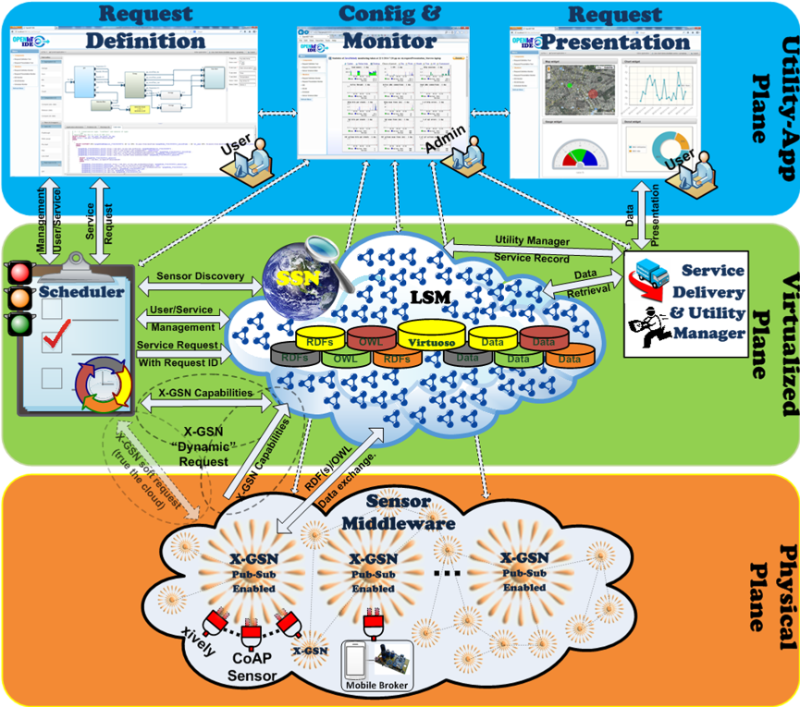
\includegraphics[scale=0.4]{images/openiot_platform1}
\caption{Arquitectura OpenIoT}\label{L400}
\end{figure}
\subsubsection*{Plano físico}
En el plano físico se encuentran los sensores. En OpenIoT se usa X-GSN como middleware para el intercambio de información entre los sensores y la nube. Este middleware se encarga de filtrar, combinar y coleccionar los datos recopilados por los sensores. X-GSN es una versión extendida de GSN, cuya principal característica es el uso de sensores virtuales. Los datos de los sensores están escritos basándose en SSN (Semantic Sensor Network), una semántica para las redes de sensores. Esto proporciona una representación que hace más fácil compartir, descubrir, integrar e interpretar los datos. Un ejemplo de esta semántica se puede ver en la figura \ref{L401} \\
\begin{figure}[H]
\centering
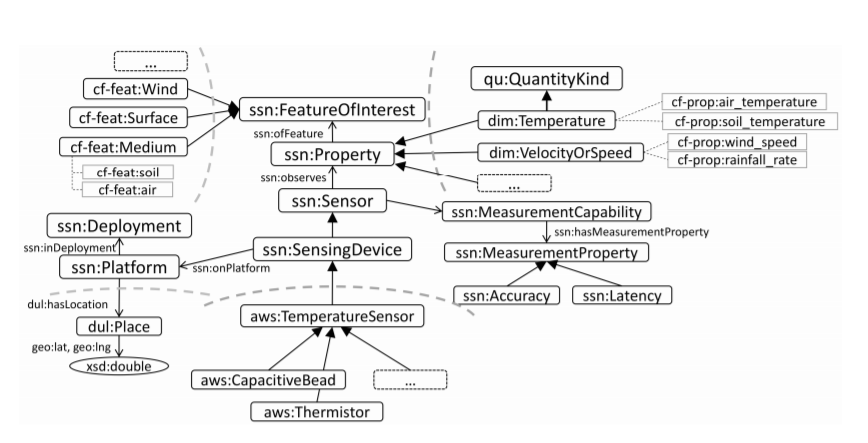
\includegraphics[scale=0.4]{images/ssn_capture}
\caption{Semántica de SSN.}\label{L401}
\end{figure}
En X-GSN se configuran los sensores usando una descripción en XML, en la que se definen los campos de los sensores. Estos campos están asociados a la semántica SSN. En la figura \ref{L404} se puede ver un ejemplo de esta descripción. \\
Para realizar el registro de sensores en la plataforma OpenIoT, es necesario que cada sensor tenga una instancia del mismo almacenada en la nube. Por ello se envía a la plataforma LSM un archivo con los metadatos del sensor, en el que se definen las propiedades del mismo. Este archivo describe los datos definidos en el archivo de configuración XML. Un ejemplo del archivo de metadatos se puede ver en la figura \ref{L402}.
\begin{figure}[H]
\centering
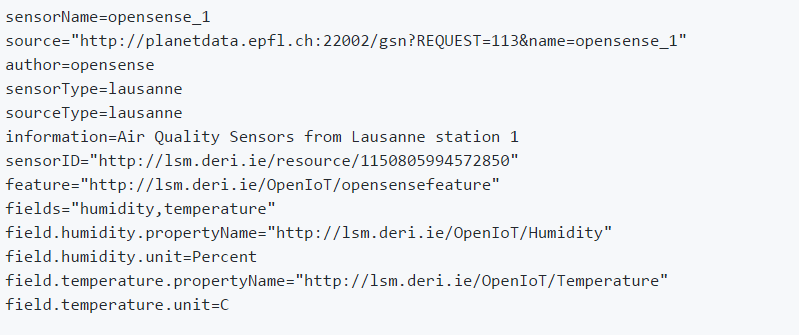
\includegraphics[scale=0.4]{images/metadata_capture}
\caption{Metadatos de un sensor.}\label{L402}
\end{figure}
En la figura \ref{L403} se puede ver el proceso para el registro de un sensor en OpenIoT. Inicialmente se crea y se configura el sensor (definición de campos, configuración del tiempo de subida ...), mediante la descripción XML (figura \ref{L404}). Posteriormente, se envía un archivo a la plataforma LSM en la nube conteniendo las propiedades del sensor. Éste se transforma en una descripción RDF, una descripción usada en la Web Semántica, que permite una representación de datos enlazados mediante la identificación de objetos (URIs), lo que facilita el descubrimiento de recursos.
\begin{figure}[H]
\centering
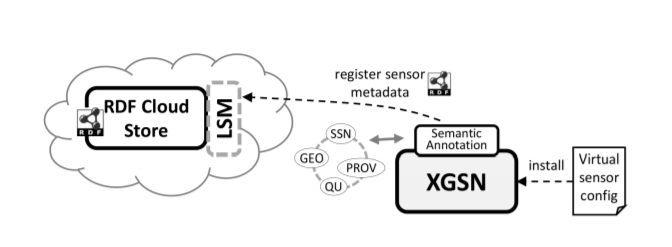
\includegraphics[scale=0.4]{images/registration_capture}
\caption{Registro de un sensor virtual}\label{L403}
\end{figure}
\begin{figure}[H]
\centering
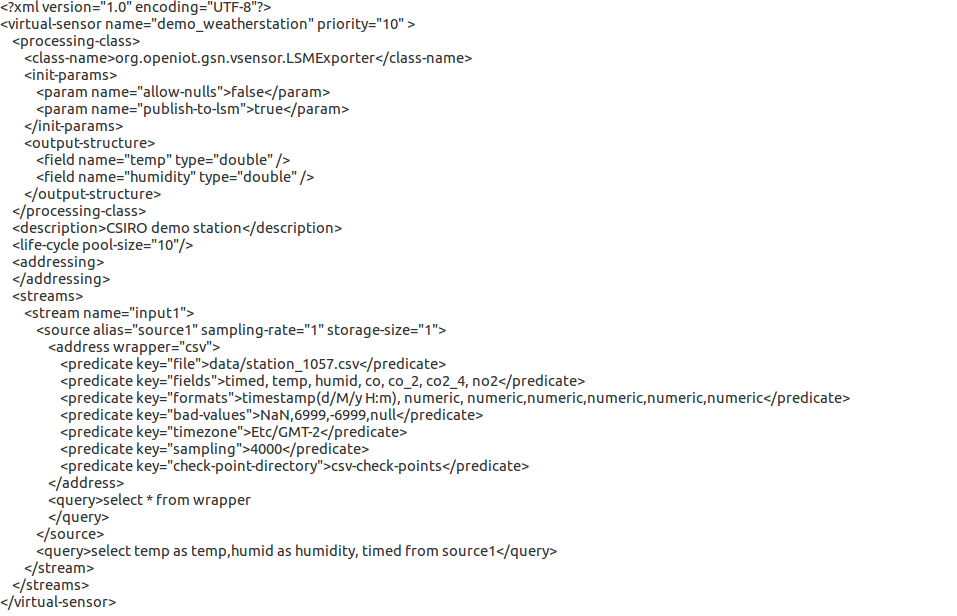
\includegraphics[scale=0.5]{images/configuration_capture}
\caption{Configuración de un sensor.}\label{L404}
\end{figure}


La colección de datos por parte de los sensores se basa en "wrappers" que coleccionan datos a través de distintos protocolos, como UDP, puerto serie, HTTP. Esto permite al usuario desarrollar y configurar el protocolo que quiera usar, lo que hace a la plataforma agnóstica respecto al hardware. Los datos se representan como flujos de listas de datos.\\
El registro de sensores en la plataforma para su posterior descubrimiento, así como la recolección de datos y su posterior almacenamiento en LSM, se hace con unos pocos archivos XML, lo que permite al desarrollador crear grandes soluciones IoT con poco esfuerzo. En la figura \ref{wrappers} se puede ver el proceso de colección y envío de datos para su almacenamiento.\\
\begin{figure}[H]
\centering
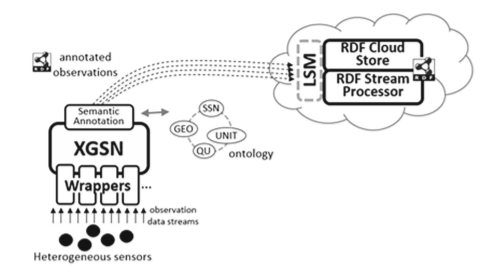
\includegraphics[scale=0.6]{images/wrappers_openiot}
\caption{Envío de datos en OpenIoT.}\label{wrappers}
\end{figure}
Por otro lado, OpenIoT ofrece también soporte para el descubrimiento y recolección de datos por parte de sensores móviles tales como pulseras, gafas, relojes y, en definitiva, sensores incluidos en dispositivos móviles. Todo esto se realiza a través de un middleware publish/subscribe para IoT llamado CUPUS (CloUd-based PUblish/Subscribe middleware). \\
CUPUS tiene dos componentes principales: 1) un agente (mobile broker, de ahora en adelante) ejecutándose en un dispositivo móvil y 2) un motor de procesado en la nube basado en publish/subscribe (cloud broker, de ahora en adelante), que se encarga del procesamiento de los datos recopilados por los sensores. CUPUS soporta el contenido basado en publish/subscribe.\\
En la arquitectura OpenIoT, los datos recopilados por los dispositivos móviles se anotan y almacenan en la nube, a través de X-GSN, de la misma forma que con los sensores estacionarios. \\

El mobile broker puede controlar los sensores conectados localmente y realizar un preprocesamiento de los datos adquiridos por los sensores y enviarlos a la nube. Además, también puede recibir publicaciones de la nube y notificar a los clientes que estén subscritos. Como se puede observar en la figura \ref{L405}, el mobile broker recibe los datos de los sensores a través de un mensaje publish y los envía al cloud broker. Pudiendo también conectarse o desconectarse del mismo.\\

El cloud broker puede enviar una notificación al mobile broker. Por otro lado, el cloud broker envía una instancia de los datos del sensor ya procesados al almacenamiento RDF, a través de X-GSN, de la misma forma que en los sensores estacionarios, tal y como se ha visto anteriormente.

\begin{figure}[H]
\centering
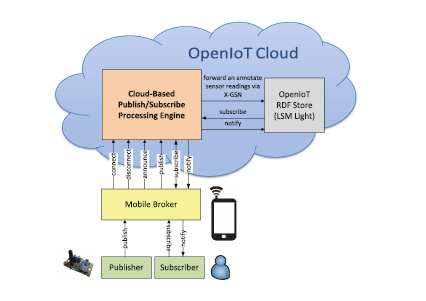
\includegraphics[scale=0.9]{images/mobilebroker_openiot}
\caption{Arquitectura publish/subscribe}\label{L405}
\end{figure}
\subsubsection*{Plano Virtual}
El plano virtual está compuesto por el almacenamiento en la nube (LSM-Light), el Scheduler y el servicio de entrega (SD\&UM). \\

LSM-Light (Linked Sensor Middleware Light) es el componente principal de OpenIoT. Es la infraestructura de almacenamiento en la nube. Esta infraestructura, además de almacenar datos y metadatos, también es capaz de ofrecer computación en la nube (software) como por ejemplo Scheduler y SD\&UM.\\ LSM considera los sensores como fuentes de entrada de datos. Los datos provenientes de los sensores se transforman en una representación de datos enlazados, como por ejemplo, RDF. Existen dos formas de importar datos en LSM: pull y push. Una es la fuente de datos (X-GSN,CoAP...) la que se encarga de enviar los datos y la otra es el propio LSM quien obtiene los datos periódicamente. LSM está compuesto por dos módulos, LSM-Client y LSM-Server. LSM ofrece funcionalidades como wrappers para la colección y visualización de datos en tiempo real, un lenguaje SPARQL para las peticiones.\\

OpenIoT usa Virtuoso, un middleware y motor de almacenamiento, que combina RDF, XML y base de datos virtuales en un solo sistema. Es el corazón de LSM-Light. \\

El scheduler se encarga de formular las peticiones realizadas por los usuarios y de acuerdo con ellas interactúa con la plataforma OpenIoT a través de la base de datos en la nube. El Scheduler tiene dos funciones prncipales: descubrir sensores y controlar los servicios. Todo esto se realiza mediante peticiones a la BBDD. Las peticiones se realizan en lenguaje SPARQL, un lenguaje usado en la web semántica para consulta de sentencias RDF. En la figura \ref{L406} se observa la Cloud DB junto con cada uno de los servicios que realiza peticiones. Request presentation y Request Definition realizan las peticiones a través de otros servicios (Scheduler y SD\&UM).\\

El Scheduler recibe las peticiones del servicio Request Definition, situado en el plano de utilidad. El Scheduler las procesa, y envía la respuesta de vuelta al plano de utilidad.\\
El SD\&UM (Service Delivery \& Utility Manager), al igual que el Scheduler, también recibe y procesa peticiones del plano de utilidad pero en este caso del servicio Request Presentation, para la presentación de los datos. Las peticiones del Scheduler y SD\&UM se realizan a la Cloud DB mediante una API.
\begin{figure}[H]
\centering
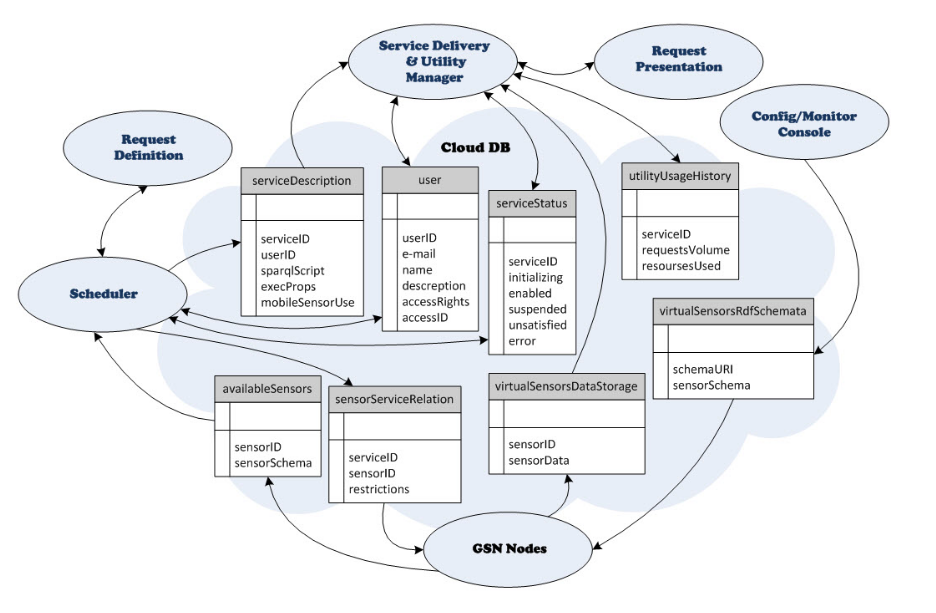
\includegraphics[scale=0.4]{images/cloud_capture}
\caption{Relación de cada servicio con la Cloud DB}\label{L406}
\end{figure}
\subsubsection*{Plano de utilidad}
En este plano se sitúan las interfaces de usuario. 
Request Definition es una aplicación que permite a los usuarios visualizar sus servicios de OpenIoT usando una interfaz basada en nodos. Cada modelo de grafos se divide en aplicaciones, siendo cada una de estas aplicaciones un conjunto de servicios que describen a la aplicación. Esto le permite al usuario controlar diferentes aplicaciones desde un solo punto. Todos estos servicios se cargan automáticamente (mediante peticiones) cuando el usuario accede a la web. Un ejemplo de esta interfaz se muestra en la figura \ref{L407}

\begin{figure}[H]
\centering
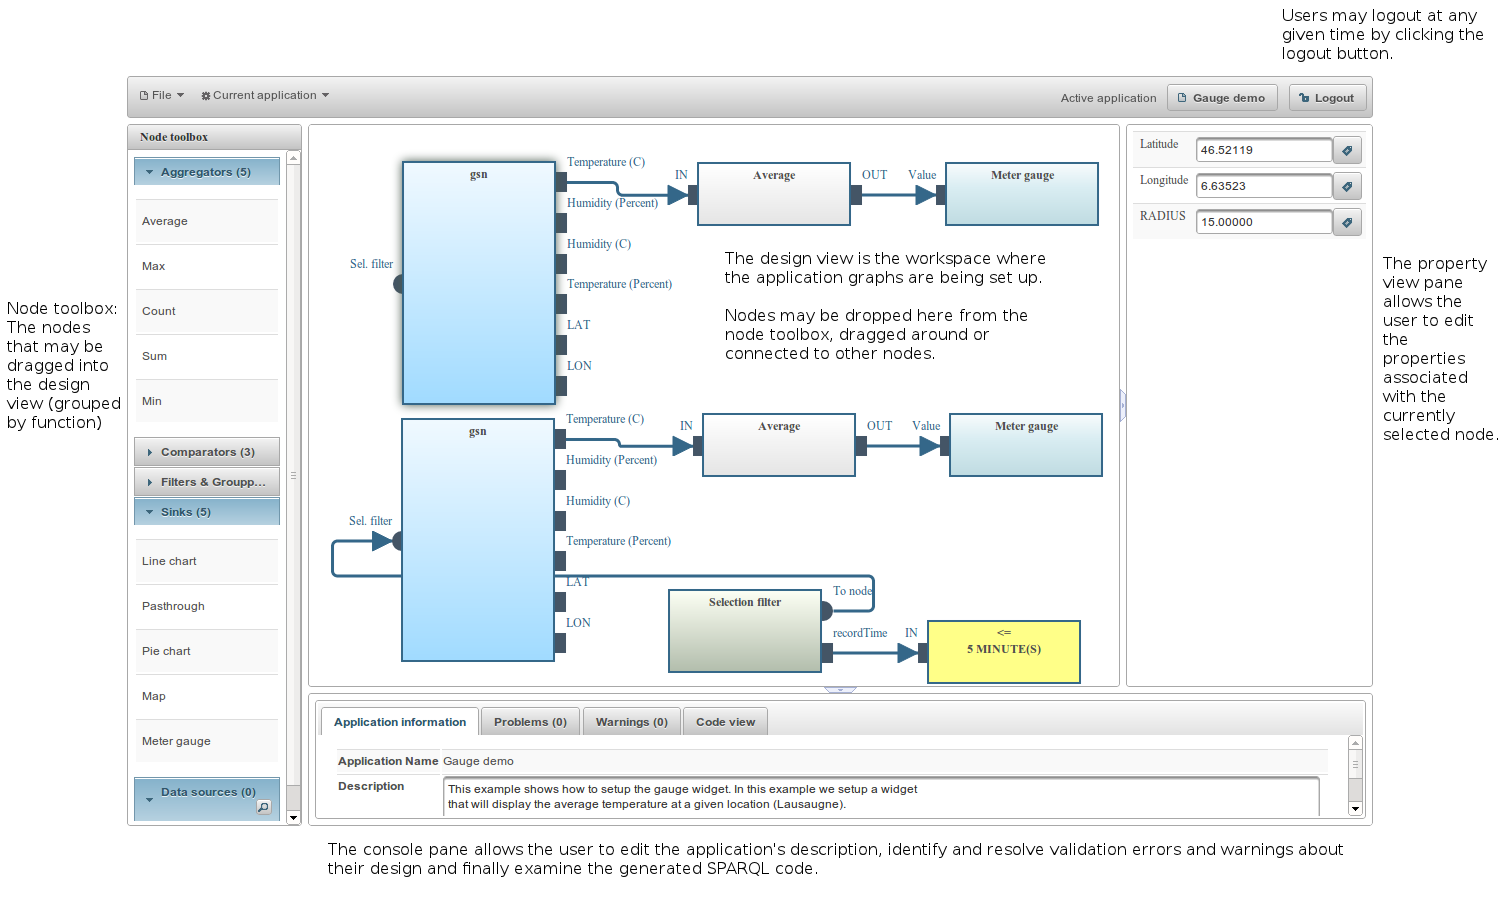
\includegraphics[scale=0.3]{images/requestDefinition}
\caption{Request Definition}\label{L407}
\end{figure}
Request Presentation es una aplicación web que proporciona al usuario una interfaz visual de los servicios que previamente ha creado en Request Definition. Obtiene la información de los nodos de Request Definition y muestra una interfaz con los datos. \\
En la figura \ref{L408} se muestra un ejemplo con la definición del servicio en Request Definition, y en la figura \ref{L409} la interfaz gráfica de los datos en Request Presentation, una vez recopilados.
\begin{figure}[H] 
\hfill
\begin{minipage}[t]{.45\textwidth}
\begin{center}
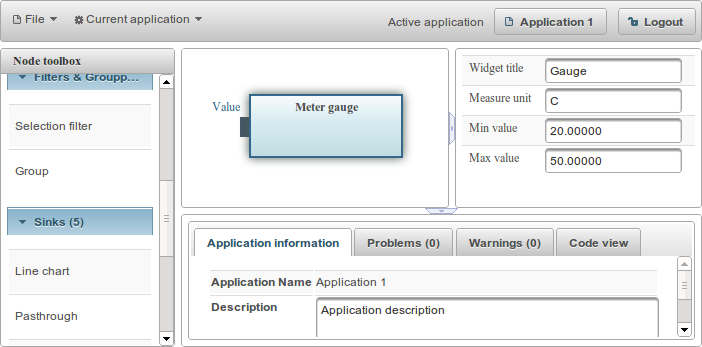
\includegraphics[width=190pt]{images/temperature_definition}
\caption{Definition}
\label{L408}
\end{center}
\end{minipage}
\hfill
\begin{minipage}[t]{.45\textwidth}
\begin{center}
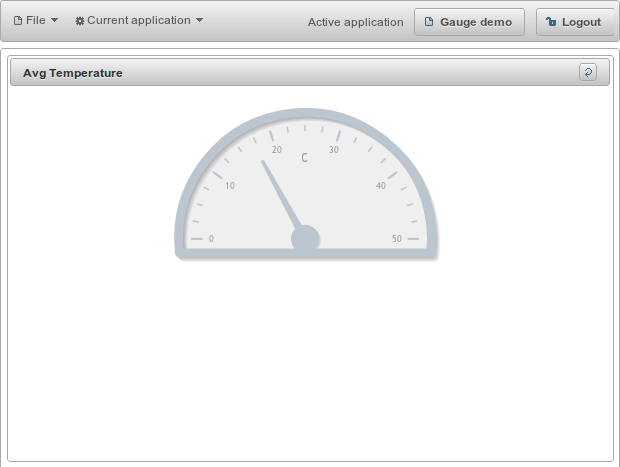
\includegraphics[width=190pt]{images/temperature_presentation}
\caption{Presentation}
\label{L409}
\end{center}
\end{minipage}
\hfill
\end{figure}

El IDE es el otro de los servicios situados en el plano de utilidad. Proporciona accesibilidad a los otros módulos o servicios de OpenIoT.
Otra de las funcionalidades que soporta IDE es la monitorización. Para implementar dicha funcionalidad se usa JavaMelody. Entre las funciones de monitorización se encuentra proporcionar datos sobre el tiempo medio de respuesta o el número de ejecuciones, la toma de decisiones ante problemas o, mostrar gráficos sobre número de sesiones, consumo de java o número de ejecuciones.

\subsection{Flujo de datos}
En base a la arquitectura que se muestra en la figura \ref{L301}, la figura \ref{L0420} representa un ejemplo del flujo que siguen los datos en la plataforma. \\
X-GSN publica los datos de los sensores virtuales basados en la configuración local de cada nodo (sensor). Paso 0. \\
Los usuarios realizan peticiones al Scheduler (paso 1) de los sensores disponibles con determinados atributos usando la interfaz Request Definition.\\
El Scheduler ejecuta (paso 2) estas peticiones (en lenguaje SPARQL) enviadas por los usuarios.\\
Una vez que tenga la respuesta (los sensores disponibles) se envía de vuelta al Scheduler (paso 3) y éste la reenvía al módulo Request Definition (paso 4), mostrándose la información al usuario.\\
El usuario, con ayuda de Request Definiton, define peticiones para  realizar determinadas reglas sobre los sensores analizados. Esta información se guarda en un objeto OSDSpec (Figura \ref{L0421}). Este objeto se envía entonces al Scheduler con la ayuda de 'registerService (paso 5).\\
El Scheduler analiza la información recibida y envía la petición al servicio necesario (paso 6).\\
Una vez que se haya configurado, el usuario puede usar el módulo Request Presentation para visualizar los datos del servicio registrado.\\
Con ayuda del SD\&UM 'getAvailableAppIDs' el Request Presentation (pasos 7,8,9 y 10) recupera todos los servicios/aplicaciones registrados de acuerdo a un usuario específico\\\
El usuario realiza una petición para recuperar los resultados relacionados con el servicio en concreto. Esto se hace enviando una petición ("pollForReport") desde Request Presentation al SD\&UM pasándole el ID de la aplicación ('application ID') (paso 11).\\
El SD\&UM realiza una petición ("getService") (paso 12) para solicitar toda la información relacionada al servicio.\\
El servicio proporciona la información al SD\&UM (paso 13).\\
El SD\&UM analiza la información, disponible en un objeto OSMO, y reenvía el script SPARQL incluido, el cual ha sido creado por Request Definition (paso 5) y almacenado por el Scheduler (paso 6), a la interfaz SPARQL del servicio (paso 14).\\
El resultado se envía al SD\&UM (paso 15) en formato SparqlResultsDoc\\El SD\&UM lo reenvía al Request Presentation (paso 16) en un objeto que incluye información de cómo esos datos se deben presentar (Figura \ref{L0422}).

\begin{figure}[H]
\centering
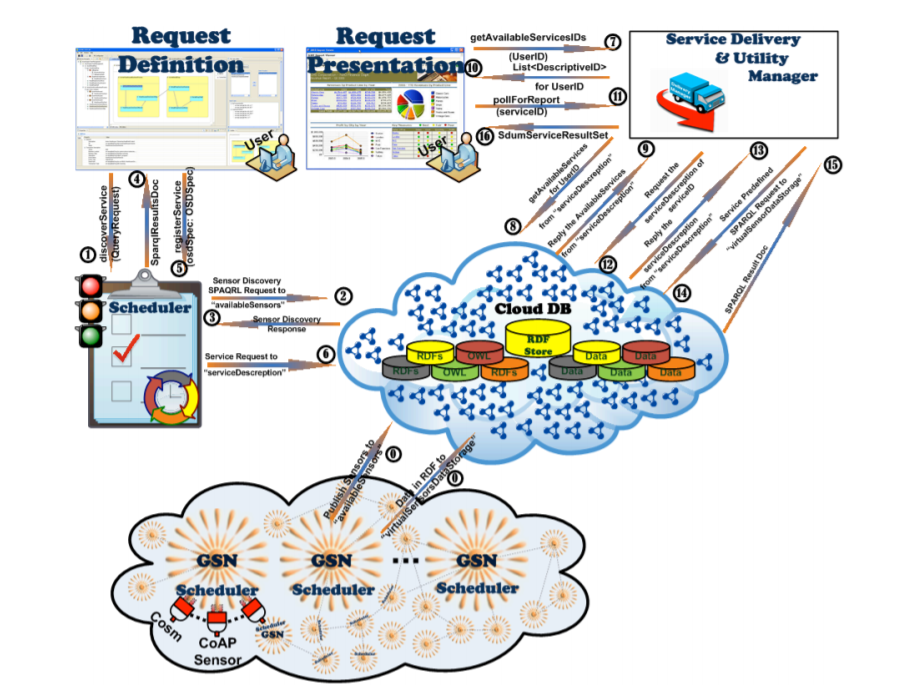
\includegraphics[scale=0.5]{images/dataFlow_capture}
\caption{Flujo de datos en OpenIoT}\label{L0420}
\end{figure}

\begin{figure}[H]
\centering
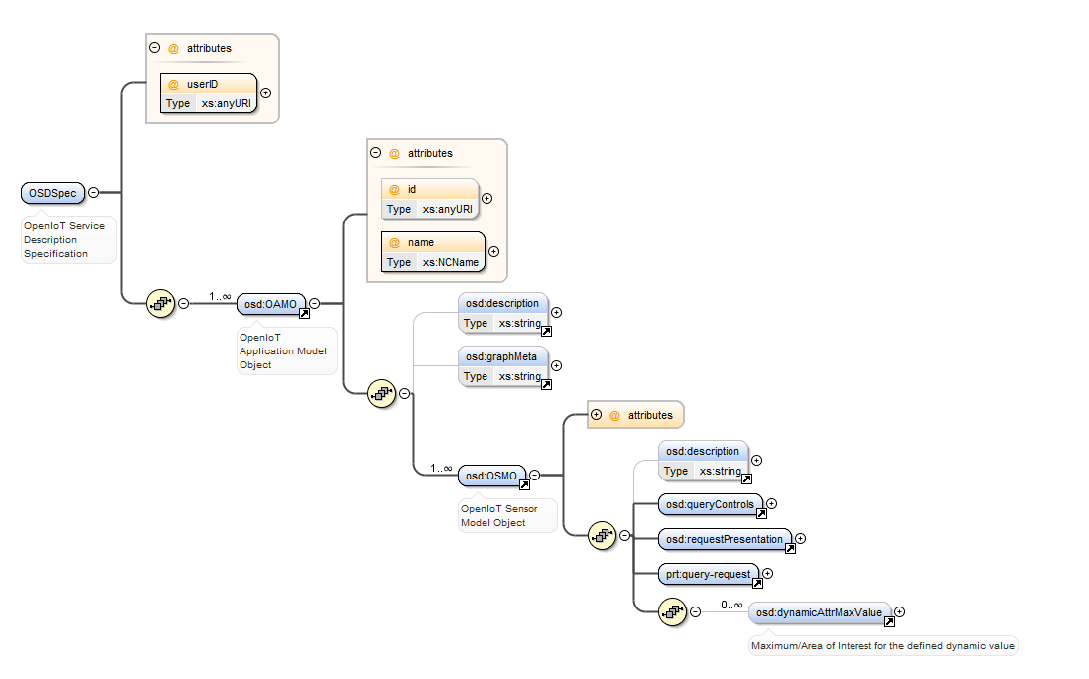
\includegraphics[scale=0.5]{images/osd_sdum}
\caption{Grafo de un objeto OSDSpec.}\label{L0421}
\end{figure}

\begin{figure}[H]
\centering
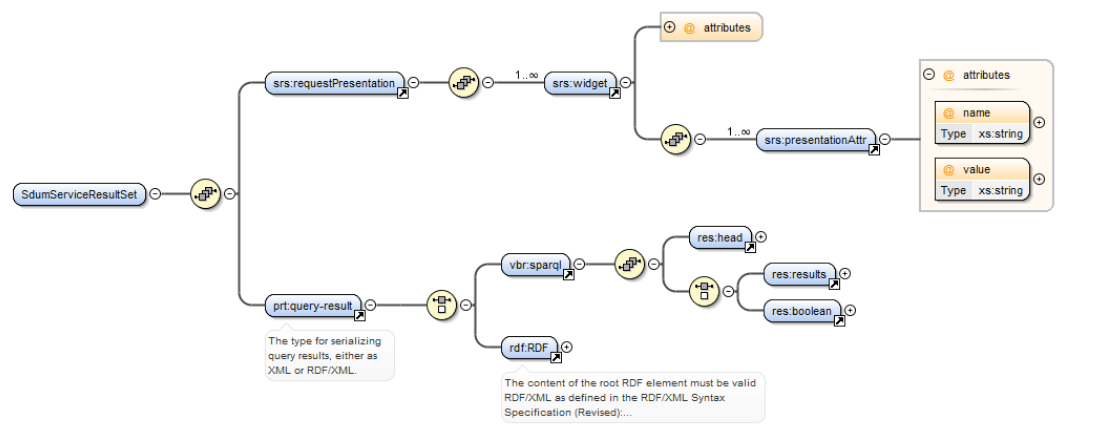
\includegraphics[scale=0.5]{images/sdum_service}
\caption{Grafo de un objeto SdumServiceResultSet.}\label{L0422}
\end{figure}

\subsubsection*{Ventajas}
En IoT cualquier cosa u objeto (TV,Smartphone...) genera una gran cantidad de eventos. Cada uno de estos objetos usa tecnologías diferentes y, desarrollar aplicaciones y servicios para controlar todo esto puede llegar a ser una tarea muy complicada. Por ello, se usan middlewares con el fin facilitar el desarrollo, proporcionando una integración entre la comunicación y la computación de los dispositivos. Entre los middleware se encuentra MAPS, TinyDB o MQTT, mencionado en el capítulo anterior.\\

A pesar de que con los middleware se facilita el desarrollo de aplicaciones en IoT, cada middleware cumple una serie de requisitos que puede que no sirvan para una determinada aplicación. Por ejemplo, en este caso, MQTT no cumplía alguno de los requisitos exigidos. No hay un middleware que reúna todas necesidades exigidas. Es aquí donde aparece OpenIoT, que permite reunir un conjunto de servicios en una única plataforma.\\

La principal ventaja de OpenIoT es la unificación de los diferentes sistemas o servicios IoT, así como el envío de datos.\\

A través de la herramienta IDE (Integrated Development Environment) Core (figura \ref{L0421} ) que ofrece OpenIoT, se puede controlar las aplicaciones IoT. Esta herramienta integra muchas de las herramientas de OpenIoT en una. Permite configurar los sensores para su integración en X-GSN (Schema Editor), monitorización del estado de los servicios IoT (SD\&UM) o definir los servicios IoT (Request Definition). Esto permite el desarrollo de aplicaciones IoT de una manera más rápida y sencilla.\\


\begin{figure}[H]
\centering
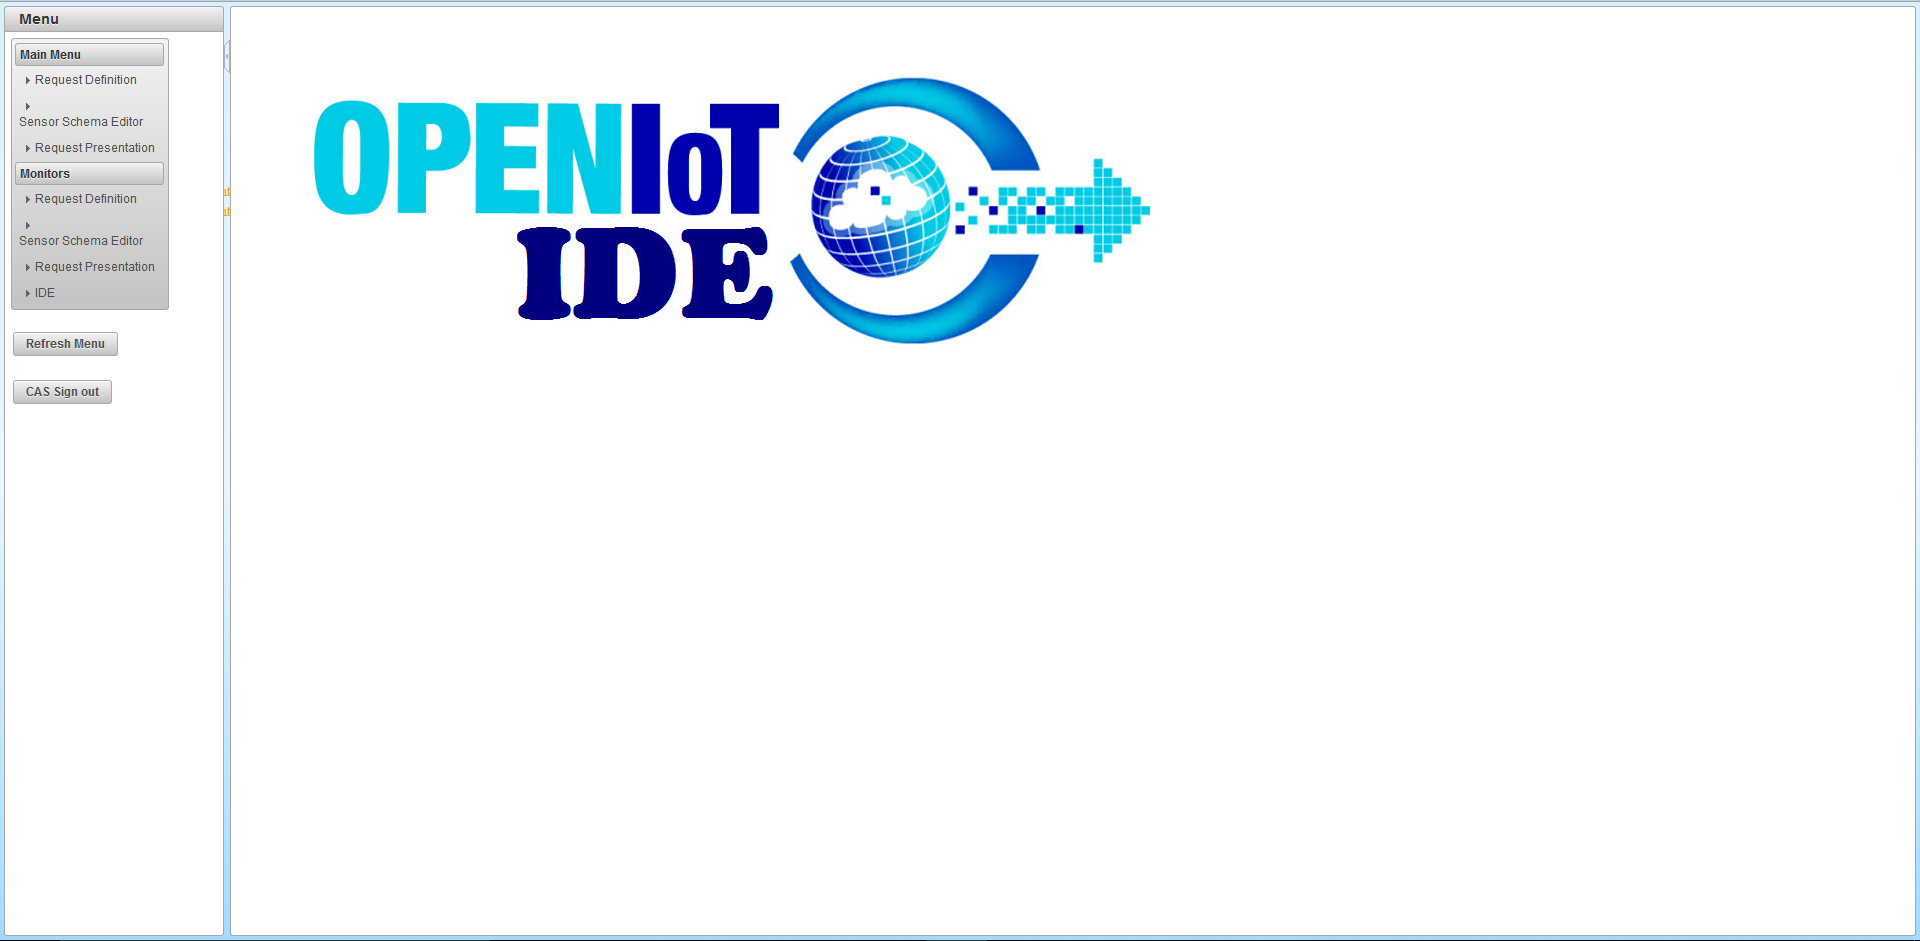
\includegraphics[scale=0.3]{images/idecore_figure}
\caption{OpenIoT IDE}\label{L0421}
\end{figure}

\begin{figure}[H]
\centering
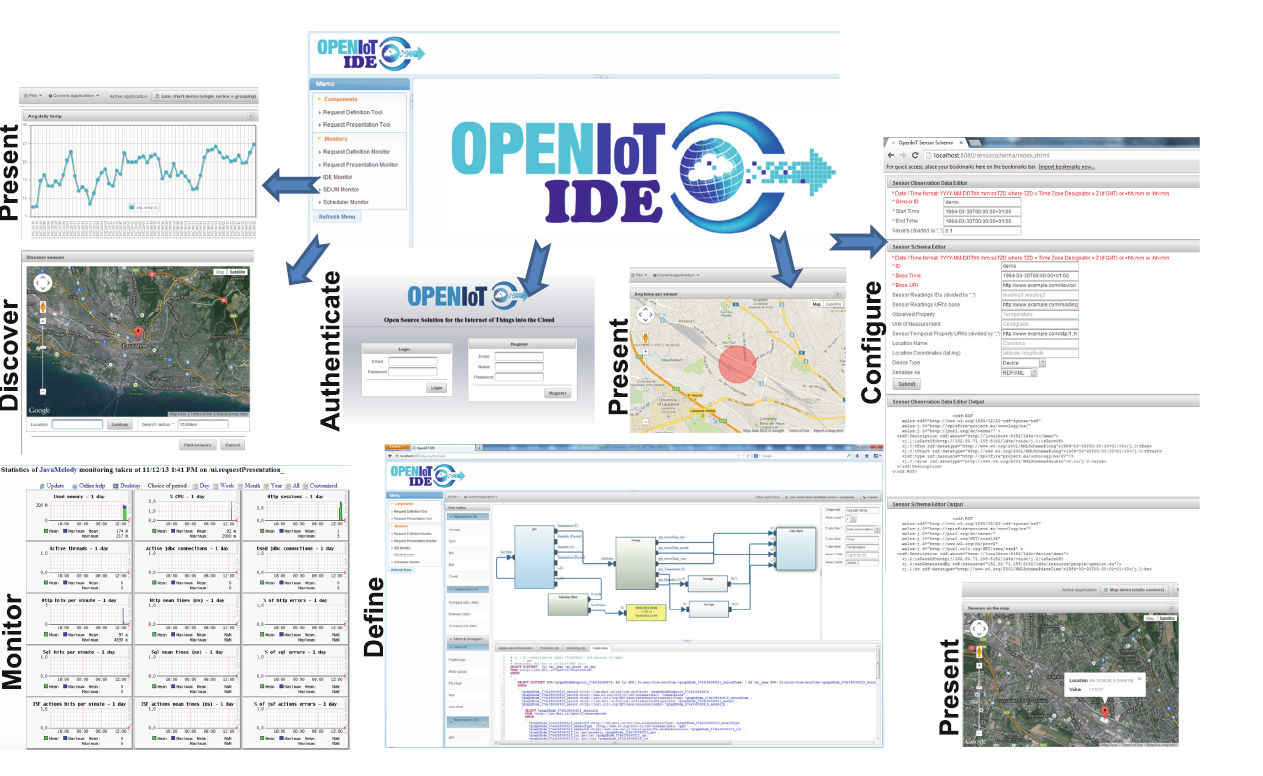
\includegraphics[scale=0.55]{images/idecoretools_capture}
\caption{Servicios integrados en IDE}\label{L0421}
\end{figure}

\section{Requisitos}
Las aplicaciones IoT deben cumplir una serie de requisitos, algunos de ellos necesarios en un entorno IoT. Algunos de estos requisitos son:


\subsection{Requisitos funcionales}
\subsubsection*{Descubrimiento de recursos}
Una de las características principales de OpenIoT es el descubrimiento de recursos. Una vez que los sensores envían su configuración a la nube a través de X-GSN, OpenIoT mediante el Scheduler, haciendo uso de la semántica SSN, es capaz de descubrir nuevos sensores o nodos.
\subsubsection*{Control de datos y recursos}
OpenIoT, a través de la herramienta SDUM, permite llevar una constante monitorización sobre los recursos. Esto permite, además de la recopilación y visualización de los datos, llevar un control sobre ellos.

\subsubsection*{Control de eventos}

\subsubsection*{Control de código}


\subsection{Requisitos no funcionales}

\subsubsection*{Escalabilidad}
OpenIoT es una plataforma totalmente escalable debido a la característica de descubrimiento de recursos que posee. Se pueden añadir nuevos nodos tan solo configurando el sensor y enviando la información sobre sus datos (metadatos) al almacenamiento en la nube. Una vez registrado el sensor, el usuario puede acceder al nuevo nodo (sensor).
\subsubsection*{Disponibilidad}
OpenIoT está formado por varios módulos/servicios, cuyo funcionamiento es responsable del funcionamiento global de la plataforma. Por ello, un fallo en alguno de los servicios (i.e el Scheduler), implica un fallo en la plataforma. 
Debido a esta dependencia, se puede decir que OpenIoT no dispone de una gran disponibilidad.
\subsubsection*{Seguridad}
La diversidad de aplicaciones interactuando en un entorno IoT hace que la seguridad sea un punto clave para poder proteger los datos. OpenIoT deja la seguridad en manos del servicio CAS (Central authorization service), encargado de la seguridad en la web.\\

La primera vez se redirecciona a los usuarios a la página de login para que se lleve a cabo una autenticación. Si esta autenticación es correcta, el CAS redirecciona al usuario a la pagina web original enviando un token. Este token se envía de un servicio a otro en cada petición y cada servicio se encarga de comprobar la validez del token.
\begin{figure}[H]
\centering
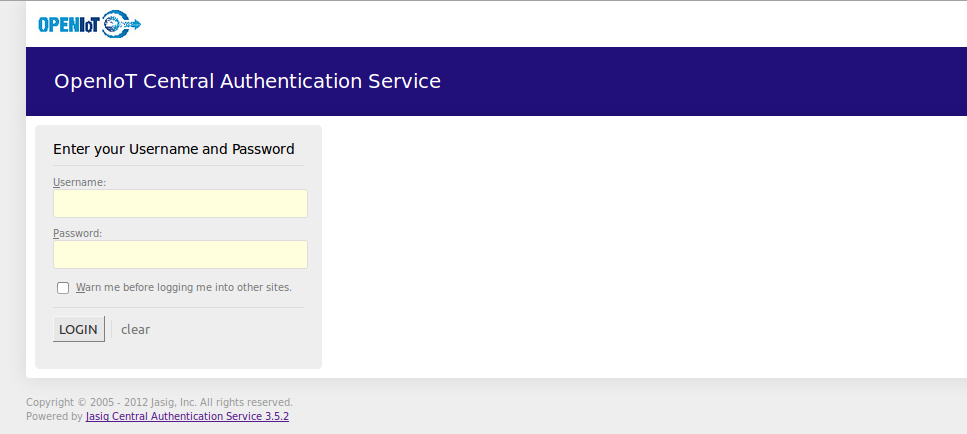
\includegraphics[scale=0.5]{images/login_capture}
\caption{Login en CAS}\label{L410}
\end{figure}
La seguridad en OpenIoT se divide en 3 módulos:
\begin{itemize}
\item[•]\textbf{Security Server:} En este módulo se usa CAS para la autenticación y autorización. Sus datos se almacenan en LSM-server. Cada cliente se tiene que registrar en CAS.
\item[•] \textbf{Security Client:} Este modulo proporciona control de acceso y autenticación. Se puede usar en aplicaciones web que interactuan con los usuarios.  
\item[•] \textbf{Security Management:} Se trata de un módulo que se usa para llevar un control sobre servicios, usuarios y permisos.
\end{itemize}
  
\subsubsection*{Tiempo real}
OpenIoT proporciona un servicio en tiempo real. El usuario a través de las interfaces de usuario puede realizar un seguimiento en tiempo real de los datos recopilados por los sensores.

\subsubsection*{Facilidad de despliegue}
Un middleware IoT debe ser fácilmente desplegable por parte del usuario. OpenIoT llegó a estar entre los 10 mejores proyectos europeos open-source del año 2013. Esta popularidad debe ayudar a mantener la plataforma totalmente actualizada por parte de la comunidad de desarrolladores e investigadores. Sin embargo, OpenIoT no cumple con este requisito ya que es una plataforma con bastantes problemas a la hora de su despliegue y además no tiene el soporte que debería para dar solución a esos problemas.

\subsection{Requisitos arquitectónicos}
\subsubsection*{Interoperabilidad}
Un middleware IoT debería funcionar en distintos dispositivos y con diferentes tecnologías. OpenIoT es una plataforma agnóstica respecto al hardware: los sensores pueden funcionar en cualquier hardware, tan solo es necesario describir los archivos de configuración y registrar los sensores en la plataforma mediante el envío de sus metadatos.  

\subsubsection*{Distribuido}






\subsubsection*{Orientado a servicio}


\subsubsection*{Adaptativo}

\subsubsection*{Abstracción de la programación}

\section{OpenIoT en la práctica}

\subsection{Casos de éxito con la plataforma}
Entre quién ha desplegado la plataforma con éxito se encuentra:
\begin{itemize}
\item[•] Universidad nacional de Irlanda - DERI
\item[•] Universidad de Zagreb - FER
\item[•] SENSAP S.A
\item[•] CSIRO
\item[•] Universidad de Estambul
\end{itemize}
\subsubsection{OpenIoT en la industria}
Cada vez más, en la industria se instalan un gran número de sensores para controlar el proceso de producción de una planta. Estos sensores generan un gran volumen de datos por lo que es necesario una solución para capturar, almacenar y procesar esos datos. SENSAP S.A (www.sensap.eu) ha desarrollado una solución basada en OpenIoT para la monitorización y seguimiento del flujo de materiales en un proceso de producción. Le permite definir y visualizar dinámicamente los KPIs (indicadores de rendimiento en la industria). En este entorno, los KPIs son el flujo de datos necesarios, los cuales son: A) recopilados por sensores físicos situados en la planta, B) transformados en el modelo de datos EPC-IS, un estándar usado en la industria, y C) transmitidos al middleware X-GSN que asegura una anotación semántica de estos datos y su posterior publicación a la nube OpenIoT. Los sensores virtuales son capaces de calcular entre otros: \\
\begin{itemize}
\item[•] Tasa de operación para un proceso específico
\item[•] Métricas de utilización de las maquinas
\item[•] Tasa de producción por tipo de producto
\item[•] Porcentaje de tiempo una operación que ha sido completada
\end{itemize} 

Una vez que se publica la información a la nube, los fabricantes son capaces de obtener y sintetizar la información de los sensores virtuales, con el fin de calcular los KPIs para los determinados procesos.\\

Para llevar a cabo este proyecto, se usó la siguiente implementación:\\
\begin{itemize}
\item[•] Sensores: Sensores físicos con el fin de calcular KPIs (tasas de operación, información de calidad...). Sensores ópticos, escáneres de códigos de barras, son algunos de los sensores utilizados en este proyecto.
\item[•] S-BOX: Productos propios desarrollados por SENSAP, para coleccionar datos de los sensores y transformarlos en eventos EPC-IS, asociados a los procesos de fabricación.
\item[•] X-GSN: Ese flujo de datos EPC-IS se envía al middleware X-GSN. Siguiendo el proceso de OpenIoT, el middleware X-GSN convierte ese flujo de datos en la anotación SSN.
\item[•] LSM: La información KPIs se envía a la nube (LSM Cloud) a través de X-GSN, tal y como marca el proceso de OpenIoT
\item[•] Visualización: Usando la herramienta Request Definition de OpenIoT, se definen servicios que calculan los KPIs asociados al proceso de fabricación. Este cálculo lo realiza a partir de los datos disponibles en el LSM Cloud. 
\end{itemize}
\subsubsection{OpenIoT en la agricultura}
Otros de los proyectos en los que se ha usado OpenIoT ha sido Phenonet, desarrollado por CSIRO. Se trata de un proyecto usado en la agricultura que permite procesar y visualizar datos del terreno en tiempo real. Esto ayuda a la toma de decisiones sobre el cultivo como, por ejemplo, planificar los recursos de agua o de nitrógeno en el cultivo y así, incrementar la eficiencia y rendimiento. La arquitectura de Phenonet se puede ver en la figura \ref{L411}
\begin{figure}[H]
\centering
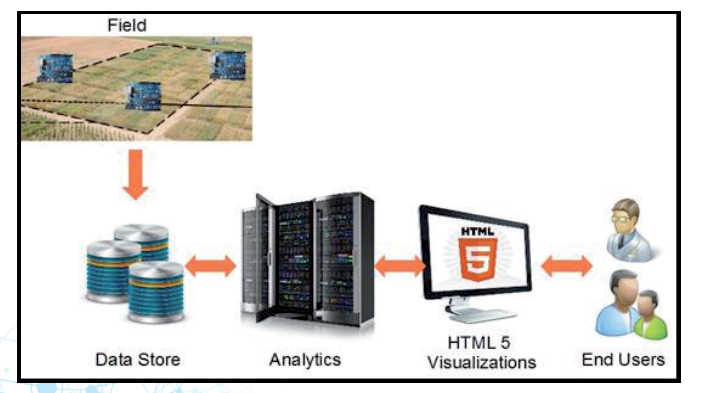
\includegraphics[scale=0.4]{images/phenonet_capture}
\caption{Arquitectura de Phenonet}\label{L411}
\end{figure}

En el campo ('field') se sitúan los sensores para medir temperatura, humedad o velocidad del viento entre otros. Los datos y metadatos se almacenan y posteriormente se procesan y analizan mediante el componente 'Data analysis'. A este componente se accede a a través de una API mediante HTML. Phenonet está basado en los siguientes módulos de OpenIoT:
\begin{itemize}
\item[•] X-GSN: Se encarga de los dato provenientes del Data Store/Field.
\item[•] Scheduler y SD\&UM: Usado para construir un experimento Phenonet en OpenIoT.
\item[•] LSM-Light: Se almacenan los datos existentes en Data Store para poder permitir el descubrimiento de sensores.
\item[•] Request Definition y Presentation: Estas herramientas se usan para el diseño. 
\end{itemize}

\section{Problemas}
Tras un tiempo intentando desplegar sin éxito la plataforma, se ha optado por descartarla. OpenIoT es una plataforma reciente y con un potencial alto pero inexplicablemente no tiene ningún tipo de soporte. Han sido muchos los problemas que se han dado a la hora de la instalación sin llegar en ningún momento a ser 100\% funcional. Tras investigar por la red nos damos cuenta que son problemas comunes que no tienen solución. Esto nos ha llevado a descartar la plataforma y buscar otra solución para el problema que planteamos.
\chapter{KAA}
\section{Introducción}
Kaa \cite{kaa}\cite{kaa_iot}\cite{code}\cite{doc} es una plataforma middleware de código abierto que, al igual que OpenIoT, busca un control e integración de las aplicaciones IoT. Se trata de un middleware que trabaja entre el hardware y las aplicaciones, ofreciendo una gran comunicación, control e interoperación entre los dispositivos conectados. Recibe soporte de la empresa KaaIoT\cite{kaa_iot}, ésta se encarga de crear soluciones haciendo uso de la plataforma, algunas de ellas muy completas y con un grado de dificultad bastante alto.
\section{Arquitectura}
Kaa tiene un poderoso back-end que facilita el desarrollo de aplicaciones en un entorno IoT. Kaa soporta múltiples plataformas en el lado del cliente, mediante puntos finales (SDKs), en diferentes lenguajes de programación. El SDK es una librería embebida en el dispositivo conectado. Esto, junto con un lenguaje de definición de datos ("data schema"), hace que Kaa sea una plataforma muy rápida y flexible. Kaa ha sido diseñada como una plataforma robusta y fácil de usar. La figura \ref{L501} muestra su arquitectura:
\begin{figure}[H]
\centering
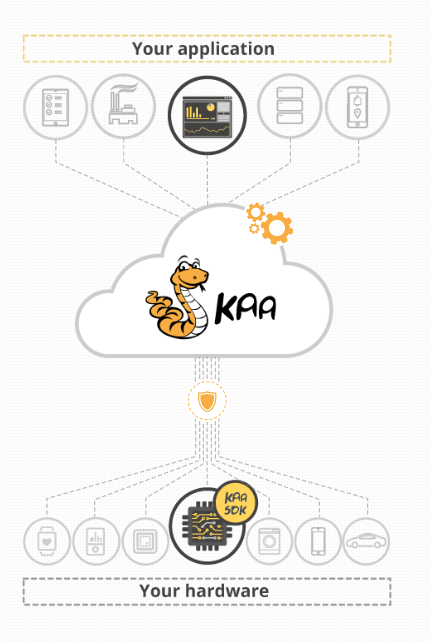
\includegraphics[scale=0.4]{images/kaa_platform}
\caption{Arquitectura Kaa}\label{L501}
\end{figure}

\subsection*{Despliegue de la plataforma}
Kaa ofrece 2 formas de despliegue, que se pueden ver en las figuras \ref{deployment1} y \ref{deployment2}.
\begin{figure}[H]
\centering
\includegraphics[scale=0.4]{images/deployment1_kaa}
\caption{Despliegue típico de Kaa}\label{deployment1}
\end{figure} 
En esta arquitectura cada uno de los endpoints tiene un SDK embebido y se comunican directamente con el servidor. Es la forma más "natural" para la que ha sido diseñada Kaa.
\begin{figure}[H]
\centering
\includegraphics[scale=0.4]{images/deployment2}
\caption{Otro despliegue con Kaa}\label{deployment2}
\end{figure} 
En esta arquitectura, uno o varios gateways o nodos centrales son los que tienen el SDK embebido. Los endpoints se comunican con el gateway a través de protocolos de transporte como Bluetooth, ZigBee o MQTT. Esta arquitectura es útil cuando no se puedan instalar el SDK en los endpoints por diferentes cuestiones (compatibilidad,bajas prestaciones...) o también cuando se quiere usar un protocolo específico de transporte. El gateway se presenta a la nube como una representación virtual del endpoint. Para versiones posteriores se plantea la inclusión de algún \MYhref{http://jira.kaaproject.org/browse/KAA-752}{framework} para simplificar la integración con Kaa en dispositivos en los que no se pueda ejecutar el SDK. Esta arquitectura tiene algunas ventajas como se verá más adelante.


\subsection*{Cluster Kaa}
El servidor Kaa se puede desplegar en un entorno de nodo único o multinodo. Cuando se habla de entorno multinodo, cada nodo representa un servidor Kaa y el conjunto de nodos interconectados representa un cluster Kaa. Por defecto, Kaa está formado por un cluster ejecutando un servidor Kaa.\\

Un Cluster requiere bases de datos SQL y NoSQL para almacenar los datos y metadatos de los endpoints. Las bases de datos relacionales se usan  las aplicaciones o grupos de endpoints y también para los metadatos. Las no relacionales almacenan todo la información relacionada con los endpoints. Kaa usa Apache Thrift\cite{apache_thrift} para la comunicación entre nodos. Cada  nodo sube información sobre la conexión, servicios activados.. y otros nodos pueden usar esta información. Para la coordinación entre ellos, Kaa usa Apache Zookeeper\cite{zookeeper}.\\

Un nodo en un cluster está ejecutando una combinación de servicios de control, operaciones y bootstrap.
\begin{itemize}
\item[•] \textbf{Servicio de control: }Es el encargado del sistema de datos, procesa llamadas de las APIs y envía notificaciones. Recibe continuamente información de Zookeeper. Para conseguir una alta disponibilidad, un Cluster Kaa tiene que incluir al menos dos nodos con el servicio de control activado. En el modo de alta disponibilidad, uno de ellos estará activo y el otro en standby, siendo zooekeeper quien se encargue de su control y activación.\\
\item[•]\textbf{Servicio de operaciones: }Es el encargado de procesar y enviar peticiones a los endpoints.\\
\item[•]\textbf{Servicio bootstrap: } Es el encargado de establecer la conexión con los endpoints. Envía información a los endpoints sobre los parámetros de conexión que pueden ser dirección IP, puerto, protocolos...
\end{itemize}
La figura \ref{cluster:kaa} representa un cluster formado por 3 nodos o servidores.
\begin{figure}[H]
\centering
\includegraphics[scale=0.6]{images/arquitectura_kaa}
\caption{Cluster Kaa}\label{cluster:kaa}
\end{figure}

Kaa proporciona una versión preconfigurada formada por un único nodo pudiéndose desplegar en local haciendo uso de VirtualBox. Otras opciones son exportarla a Amazon Web Services o instalar manualmente un servidor Kaa, pudiéndolo hacer en un entorno de un solo nodo o multinodo.\\

Kaa es multi-entidad (Tenant) y un cluster puede soportar varias de ellas. Una aplicación en Kaa tiene que pertenecer a un Tenant y los endpoints se registran en las aplicaciones. Para distinguir los endpoints se usan perfiles de endpoints además de un identificador único. Con los perfiles de endpoints se pueden crear grupos de endpoints como se verá más adelante.
\begin{figure}[H]
\centering
\includegraphics[scale=0.3]{images/tenants}
\caption{Entidades y grupos de endpoints en Kaa}\label{tenant:kaa}
\end{figure}


\textbf{Nota: Se ha analizado la versión 0.10, la última hasta la fecha de publicación de este documento.}
\section{Funcionamiento}
La figura \ref{flujo_kaa} muestra un flujo de datos en Kaa. Los endpoints recogen datos y, a través del SDK, se envían al servidor. El SDK dependerá de la plataforma y del lenguaje de programación. El envío de datos al servidor desde el SDK se realiza en un formato común, cuyo contenido se define previamente en el servidor mediante los "Log Schemas". \\
Kaa, como plataforma Cloud-IoT que es, almacena esos datos para que puedan ser procesados y analizados posteriormente. Kaa no ofrece un análisis de los datos como sí ofrecía OpenIoT, si no que tan solo ofrece una persistencia de los datos, sin embargo es posible integrarla con otros sistemas (p. ej. Spark o Zeppelin) para realizar un análisis de los datos. Kaa ofrece tanto bases de datos relacionales como no-relacionales para el almacenamiento. MariaDB y MongoDB , relacional y no-relacional respectivamente, son las bases de datos por defecto usadas por Kaa. Algunas funciones como las notificaciones no se les puede aplicar una persistencia de datos. En su lugar se define el tiempo de vida (TTL) y así los dispositivos pueden recibirla en caso de que estén offline en el momento del envío. Una vez pasado ese TTL, se elimina. 
\begin{figure}[H]
\centering
\includegraphics[scale=0.4]{images/kaa_platform1}
\caption{Flujo de datos en Kaa}\label{flujo_kaa}
\end{figure} 
\subsection*{Roles}
En Kaa existen 3 roles diferentes que son asignados a los usuarios:
\begin{itemize}
\item[•] \textbf{Kaa administrador:} Es el administrador más alto en Kaa. Tiene derechos para crear, editar y eliminar Tenant administradores.
\item[•] \textbf{Tenant administrador:} Usuario con permisos para configurar las aplicaciones, usuarios y familias de clases de eventos dentro de una entidad Tenant.
\item[•] \textbf{Tenant desarrollador:} Usuario que crea y controla perfiles de aplicaciones. Los usuarios con rol de Tenant desarrollador pueden crear y configurar esquemas, grupos de endpoints y notificaciones. Es quien crea el SDK.
\end{itemize}
La versión preconfigurada de VirtualBox ofrece unos credenciales por defecto para cada usuario.
\subsection*{Registro de endpoints}
Para funcionar en un cluster Kaa, todos los endpoints tienen que registrarse haciendo uso de credenciales de seguridad y el perfil endpoint. En el proceso de registro, los endpoints primero se comunican con los servicios bootstrap para obtener una lista de servicios de operaciones. Una vez recibida, se comunica con el servicio de operación en concreto para enviar los datos del endpoint (esto es, ID y perfil de endpoint). El proceso de registro se muestra en la figura \ref{registration}:
\begin{figure}[H]
\centering
\includegraphics[scale=0.25]{images/registration}
\caption{Proceso de registro de endpoint en Kaa.}\label{registration}
\end{figure} 

El identificador del endpoint dentro de una aplicación es el Hash de su clave pública, generada automáticamente en el primer registro. Si los credenciales no son válidos, Kaa no iniciará la sesión. Al crear la aplicación, ésta se asigna a un credencial de servicio. Estos credenciales son:
\begin{itemize}
\item[•] \textbf{Trustful:} Implementación por defecto y permite a cualquier endpoint registrarse y conectarse al cluster. 
\item[•] \textbf{Internal:} Solo permite conectarse al cluster a una lista de endpoints en concreto, previamente suministrada al servidor. 
\end{itemize}
Kaa también permite crear credenciales de servicio personalizados.

\subsection*{Esquemas en Kaa}
Kaa ha sido diseñada para ser una plataforma sencilla de usar, por ello la configuración en el lado del servidor se realiza mediante esquemas, basados en Apache Avro\cite{avro}. El desarrollador (esto es, tenant desarrollador) es el encargado de definir estos esquemas. Son usados para la configuración de notificaciones, eventos, colección de datos ... Un ejemplo de estos esquemas es:
\begin{lstlisting}[language=json]
{ 
    "type":"record",
    "name":"ExampleNotification",
    "namespace":"org.kaaproject.kaa.schema.sample.notification",
    "fields":[ 
        { 
            "name":"message",
            "type":"string"
        }
    ]
}
\end{lstlisting}
\section{Qué ofrece Kaa}
Evaluando a Kaa como middleware IoT, se puede decir que cumple con una gran cantidad de requisitos esenciales. Se va a evaluar como el resto de middleware analizados, es decir, mediante la evaluación de los requisitos presentes en la tabla de la figura \ref{L105} 
 
\subsection{Requisitos funcionales}
\subsubsection*{Descubrimiento de recursos}
Kaa desplegada como la arquitectura mostrada en la figura \ref{deployment2} permite un descubrimiento de nuevos dispositivos a través del Gateway. El Gateway es un dispositivo que actúa como puente entre los endpoint y la nube, siendo el gateway quien tiene el SDK embebido. El Gateway se puede diseñar para que avise a Kaa cuando se conecte a él un nuevo dispositivo. 


Kaa, con la arquitectura típica, no ofrece un descubrimiento de recursos como tal, pero mediante el sistema de eventos se puede conseguir tal propósito. Estos eventos se generan en los endpoints y, al igual que el almacenamiento de datos, se definen mediante esquemas. La figura \ref{L506} muestra un diagrama de cómo se generan y procesan los eventos. Haciendo uso de ellos, se puede avisar al resto de endpoints de la aparición de un nuevo recurso (endpoint).
\begin{figure}[H]
\centering
\includegraphics[scale=0.5]{images/events_schema}
\caption{Diagrama de eventos en Kaa}\label{L506}
\end{figure} 
\subsubsection*{Control de recursos}
En IoT se busca que los recursos puedan ser controlados para que, por ejemplo, se pueda reaccionar ante un fallo de éstos. Kaa no ofrece un control de recursos como tal, pero haciendo uso de los eventos y notificaciones se puede conseguir tal propósito. Por ejemplo, una solución sencilla podría ser que un endpoint guarde cada 5/10 min un valor característico, como su timestamp y, mediante un sistema de análisis, analizar los datos y, en caso de fallo, enviar un evento o notificación a un endpoint en concreto, que será el encargado de reaccionar ante tal efecto.\\
Otro ejemplo podría ser implementar en un SDK una función 'ping' a la que, haciendo uso del sistema de eventos de kaa, tengan que responder todos los endpoints en un determinado tiempo, si no lo hacen se podría considerar como endpoint caído y actuar ante tal efecto.\\
Por tanto, el sistema de eventos y notificaciones es un sistema completo con el que se pueden realizar muchas funciones. Toda funcionalidad tendrá que ser implementada en los endpoints, donde podrán ser conectados a servidores para realizar funciones más complejas. El motivo por el cual se usa Kaa es, sin duda, su robustez y heterogeneidad con distintas plataformas así como su facilidad de uso. 

\subsubsection*{Control de datos}
Los datos son la principal característica de las aplicaciones IoT, cuando se habla de datos se hace referencia principalmente a los recopilados por los sensores. Un procesamiento, almacenamiento así como una monitorización o filtrado de datos es fundamental para poder desarrollar una aplicación IoT. \\ 

Kaa, a diferencia de otras plataformas comerciales, no ofrece un procesamiento o visualización de datos. En kaa tan solo se almacenan los datos provenientes de sensores. A pesar de que no ofrezca herramientas de análisis de datos como tal, se pueden usar herramientas externas. \\
Con estas herramientas se recopilan los datos almacenados en Kaa de manera que sean estas herramientas las que gestionen y analicen los datos. Para comunicarse con los EndPoints se usan las notificaciones Kaa mediante su API.
Más adelante se verá un ejemplo práctico sobre ésto, en el que se ha usado Apache Zeppelin como herramienta para el análisis de datos y Cassandra como base de datos de Kaa. Una vez analizados, si supera un cierto umbral, se envía una notificación a Kaa para que encienda un LED en la raspberry.
En la figura \ref{L507} se puede ver un esquema de uso con Apache Storm.
\begin{figure}[H]
\centering
\includegraphics[scale=0.6]{images/esquema_apache}
\caption{Esquema de uso para la monitorización de datos con Apache Storm}\label{L507}
\end{figure} 
\subsubsection*{Control de eventos}
-------------
\subsubsection*{Control de código}
-------------
//////////////////////////////////Una de las principales características de Kaa es que es Open Source con todo lo que ello implica. El código es totalmente transparente al usuario.
\subsection{Requisitos no funcionales}
\subsubsection*{Escalabilidad}
La plataforma Kaa ha sido diseñada para ser escalable horizontalmente. Se pueden añadir miles de endpoints al mismo nivel, es decir, no puede haber varios niveles en la jerarquía. Para poder agrupar distintos endpoints se puede hacer uso de los grupos de endpoints (endpoint group). 
\begin{figure}[H]
\centering
\includegraphics[scale=0.6]{images/endpoint_group.png}
\caption{Grupos de Endpoints}\label{L508}
\end{figure}
\subsubsection*{Tiempo real}
Kaa es un sistema en tiempo real, entendiendo tiempo real como unos ms de retraso. Ya que Kaa, por defecto, usa HTTP sobre TCP para la comunicación entre SDK y Cluster, por tanto, por definición, es un servicio con retardos, aunque despreciables para el escenario que se plantea.\\  Kaa es agnóstica respecto al transporte, para un mismo endpoint se pueden usar diferentes protocolos de transporte. Para escenarios en los que la característica de tiempo real pueda marcar la diferencia entre éxito y fracaso, se puede usar UDP como protocolo de transporte.


\subsubsection*{Disponibilidad}
La arquitectura horizonal y lineal de Kaa hace que no cuente con ningún punto de fallo. Esto junto con la conexión entre los cluster, dota al sistema con una alta disponibilidad.  Además, los datos de los endpoints se almacenan en bases de datos tolerantes a fallos. Esta interconexión entre los nodos, hace que sea necesario un balanceo de carga para no sobrecargar la red. Kaa usa un balanceo activo para redireccionar el tráfico entre los distintos nodos según el tráfico de de cada uno de ellos. Para la coordinación entre los diferentes nodos se usa Apache Zooekeeper.
\begin{figure}[H]
\centering
\includegraphics[scale=0.5]{images/disponibilidad_captura}
\caption{Esquema Zooekpeer en Kaa}\label{L509}
\end{figure} 

\subsubsection*{Seguridad y privacidad}
Por defecto, en la comunicación entre Kaa y el SDK se usa una encriptación con 2048-bit RSA y AES-256. Kaa también asegura un almacenamiento de datos seguro en la base de datos así como la autenticación en la plataforma. Cada vez que se inicia una nueva sesión, cada endpoint envía una clave AES generada de forma aleatoria y encriptada con la clave pública del nodo Kaa que gestiona la sesión. 
Esta clave está firmada digitalmente con la clave privada del endpoint. Kaa usa el hash SHA-1 de la clave pública como identificador del endpoint en el sistema.
\begin{figure}[H]
\centering
\includegraphics[scale=0.5]{images/security_capture}
\caption{Seguridad en Kaa}\label{L510}
\end{figure} 
\subsubsection*{Facilidad para su despliegue} 
Kaa es un middleware que ofrece facilidades para su desarrollo. Dispone de una versión en una maquina virtual ya preconfigurada con aplicaciones y ejemplos de uso de la plataforma. El uso de SDKs facilita la interoperabilidad de diferentes plataformas sin la intervención del usuario. Con Kaa se consigue que el desarrollador se 'olvide' de la parte del servidor.
\subsubsection*{Popularidad}
Kaa es un middleware reciente y con mucho soporte y documentación, lo que facilita su despliegue.
\subsection{Requisitos arquitectónicos}
\subsubsection*{Interoperabilidad}
La interoperabilidad entre distintas plataformas es una de las características de Kaa, en la que una misma aplicación puede ser desarrollada para diferentes plataformas, tan solo descargando el SDK generado por el servidor. Para conectar un endpoint a la plataforma será necesario compilar este SDK en el dispositivo junto a la aplicación desarrollada. Esto hace que sea una plataforma totalmente heterogénea en cuanto a plataformas se refiere. Un endpoint puede ser ejecutado en distintos dispositivos, desde un teléfono móvil a una raspberry o arduino, debido al bajo procesamiento que requiere (10KB de RAM y 40KB de ROM para el caso de C). 
\begin{table}[H]
\centering
\caption{Compatibilidad entre SDKs y plataformas}
\label{table:platform_supported}
\begin{tabular}{l|c|c|c|c|}
\cline{2-5}
                                   & C      & C++    & Objetive - C & Java   \\ \hline
\multicolumn{1}{|l|}{Linux}        & \cmark & \cmark &              & \cmark \\ \hline
\multicolumn{1}{|l|}{Windows}      &        & \cmark &              & \cmark \\ \hline
\multicolumn{1}{|l|}{Android}      &        &        &              & \cmark \\ \hline
\multicolumn{1}{|l|}{iOS}          &        &        & \cmark       &        \\ \hline
\multicolumn{1}{|l|}{Raspberry Pi} & \cmark & \cmark &              &        \\ \hline
\end{tabular}
\end{table}


\subsubsection*{Distribuido}
Kaa es una plataforma distribuida, que se organiza en clusters donde cada uno de ellos puede ejecutar una determinada funcionalidad que será controlada como un único sistema. Por defecto, Kaa está formada por un único cluster ejecutando el servidor Kaa. 




\subsubsection*{Abstracción de la programación}
Kaa proporciona una interfaz al desarrollador, posibilitando una sencillez a la hora de crear las aplicaciones. El desarrollador tan solo tiene que crear los esquemas de datos, pues la plataforma se encarga de generar el código. Además de la interfaz, Kaa proporciona una API que permite realizar, mediante llamadas a la misma, todas las funciones que se pueden llevar a cabo a través de la interfaz y así, pueden ser los endpoints quienes realicen una determinada tarea.
\subsubsection*{Basado en servicio}
-----

\subsubsection*{Autónomo}

\subsubsection*{Adaptativo}
Un middleware IoT debe adaptarse a los cambios que se produzcan en su entorno, como pueda ser el cambio en la red.\\Kaa soporta virtualmente cualquier protocolo de red, endpoint o almacenamiento de datos, lo que hace a la plataforma tolerante a cambios.



\section{Uso de la plataforma}
\subsection{Instalación}
Como se ha comentado, existen 2 formas de instalar la plataforma, bien desplegar en local la plataforma haciendo uso de la versión ya preconfigurada para VirtualBox y la que incluye algunos ejemplos, o bien, construir un servidor propio haciendo uso del código fuente disponible en el GIT de Kaa. También se puede desplegar la versión preconfigurada en Amazon Web Services. Todo esto está perfectamente documentado en la web de Kaa.
\subsection{Partes de la plataforma}
Las características de Kaa son:
\subsubsection*{Eventos}
Kaa proporciona un mecanismo para la entrega de eventos (mensajes) a través de los endpoints. Los eventos pueden ser unicast o multicast, eligiendo así el/los destinatario/s. Los endpoints generan los eventos y los envían al Kaa server, éste se encarga de enviarlos a los endpoints acorde al esquema de eventos, previamente configurado por el desarrollador. La figura \ref{L505} muestra el proceso de envío y recepción de eventos.\\
En el siguiente ejemplo se muestra la definición de un esquema de eventos. El formato está basado en \MYhref{http://avro.apache.org/docs/current/spec.html}{Avro Schema}.
\begin{lstlisting}

{
    "namespace": "com.company.project",
    "type": "record",
    "classType": "event",
    "name": "SimpleEvent2",
    "fields": [
        { "name": "field1", "type": "int"},
        { "name": "field2", "type": "string"}
    ]
}

\end{lstlisting}
Cada evento se basa en una clase en concreto (EC), definida en el esquema de eventos. Una EC se identifica mediante su nombre completo, en el ejemplo de arriba sería: " com.company.project.SimpleEvent2". El identificador es único y no puede haber 2 ECs con el mismo nombre en el mismo tenat ////////////////////////explicar tenat///////////.\\

Por otra parte, las clases de eventos (ECs) se agrupan en familias de clases de eventos (ECFs). Un ECF se identifica por su nombre y/o nombre de clase, por lo que no puede haber 2 ECFs con el mismo nombre o nombre de clase en un mismo tenat. El siguiente esquema muestra un ejemplo de definición de ECF:
\begin{lstlisting}
[
    {
        "namespace": "com.company.project.family1",
        "name": "SimpleEvent1",
        "type": "record",
        "classType": "event",
        "fields": []
    },
    {
        "namespace": "com.company.project.family1",
        "name": "SimpleEvent2",
        "type": "record",
        "classType": "event",
        "fields": [
            { "name": "field1", "type": "int" },
            { "name": "field2", "type": "string" }
        ]
    }
]
\end{lstlisting}
\subsubsection*{Colección de datos}
Los endpoints almacenan datos recopilados ("log") siguiendo una estructura predefinida. El SDK implementa la subida de 'logs' desde los endpoints al servidor. El servidor lo almacena en bases de datos. En el siguiente ejemplo se muestra un simple esquema de almacenamiento de datos (log schemas), compatible con \MYhref{http://avro.apache.org/docs/current/spec.html}{Avro Schema}:
\begin{lstlisting}
{
    "name": "LogData",
    "namespace": "org.kaaproject.sample",
    "type": "record",
    "fields": [
    	{
            "name": "tag",
            "type": "string"
        },
        {
            "name": "message",
            "type": "string"
        }
    ]
}
\end{lstlisting}
La especificación de la base de datos se hace mediante log appenders usando la interfaz de usuario. 
\subsubsection*{Perfiles y grupos}\label{sec:grouping}
Kaa permite la agrupación de endpoints pertenecientes a la misma aplicación, en grupos de endpoints. Estos grupos se controlan de forma independiente, para ello se usan filtros de perfiles (profile filter (PF), en inglés) asignados a un determinado grupo. Los endpoints cuyos perfiles coincidan con los filtros de perfiles asociados al grupo, se registrarán automáticamente como miembros de ese grupo. Los filtros son expresiones que definen algunas características de los miembros del grupo. Se pueden asignar varios perfiles a un grupo.\\
A cada grupo de endpoints dentro de una aplicación se le asignan diferentes pesos. Este valor se usa para la prioridad de cada grupo, siendo el valor más grande el que mayor prioridad tiene. Por defecto, hay un grupo "all" cuyo peso es 0. Este grupo contiene todos los endpoints registrados en la aplicación.  \\

Los endpoints envían sus perfiles al servidor durante su registro.  Además de los perfiles enviados por los endpoints (lado del cliente), se pueden definir perfiles en el lado del servidor. Con todos estos datos, el servicio de operaciones de Kaa clasifica los endpoints dentro de grupos basados en los filtros. 
\begin{figure}[H]
\centering
\includegraphics[scale=0.4]{images/filters}
\caption{Uso de perfiles de grupos de endpoints en Kaa}\label{L508}
\end{figure}
Los PF están basados en \MYhref{http://docs.spring.io/spring/docs/3.0.x/reference/expressions.html}{Spring Language}. Los filtros se evalúan usando 3 variables de contexto:
\begin{itemize}
\item[•] "cp" - Perfil de endpoint en el lado del cliente
\item[•] "sp" - Perfil de endpoint en el lado del servidor
\item[•] "ekh" - Hash del endpoint 
\end{itemize}
Al definir los filtros se le asignan los esquemas de perfiles de endpoints, tanto del lado del cliente como del servidor. Estos filtros estarán relacionados con dichos esquemas.\\

Un ejemplo de esquema en el lado del cliente podría ser:
\begin{lstlisting}[language=json,firstnumber=1]
[  
   {  
      "name":"ClientSideEndpointProfileChild",
      "namespace":"org.kaaproject.kaa.common.endpoint.gen",
      "type":"record",
      "fields":[  
         {  
            "name":"otherSimpleField",
            "type":"int"
         },
         {  
            "name":"stringField",
            "type":"string"
         }
      ]
   }
]
\end{lstlisting}
Y en el lado del servidor:
\begin{lstlisting}[language=json]
[  
   {  
      "namespace":"org.kaaproject.kaa.common.endpoint.gen",
      "type":"record",
      "name":"ServerSideEndpointProfile",
      "fields":[  
         {  
            "name":"simpleField",
            "type":"string"
         },
         {  
            "name":"arraySimpleField",
            "type":{  
               "type":"array",
               "items":"string"
            }
         }
      ]
   }
]
\end{lstlisting}
Un ejemplo de filtro asociado a dichos esquemas puede ser:\\

\framebox{\parbox{\dimexpr\linewidth-4\fboxsep-4\fboxrule}{\itshape \#cp.recordField.otherSimpleField==123\\
\#sp.arraySimpleField[0]=='SERVER\_SIDE\_VALUE\_1'}}
\subsubsection*{Notificaciones}
Kaa dispone de un sistema de notificaciones para la entrega de mensajes desde el clúster Kaa hasta los endpoints. La estructura de los datos se define en el esquema de notificaciones, configurado en el servidor y desplegado dentro de los endpoints. Las notificaciones a tópicos de forma que para recibir una notificación, el endpoint tiene que subscribirse a uno o varios tópicos. También, se puede asignar un tópico a todo un grupo de enpoints. El envío de notificaciones se puede hacer mediante la interfaz de usuario o mediante una llamada a la API. 
\begin{figure}[H]
\centering
\includegraphics[scale=0.5]{images/notifications}
\caption{Notificaciones en Kaa}\label{L508}
\end{figure}
\subsubsection*{Distribución de datos}
La distribución de datos es una de las principales características de Kaa ya que los desarrolladores pueden definir cualquier tipo de datos mediante los esquemas de Kaa.
\subsubsection*{Propiedad de los Endpoints}
En Kaa, los usuarios pueden asociar Endpoints a propietarios. Estos propietarios pueden ser personas, grupos de personas o organizaciones. Para capturar o añadir un endpoint a un propietario se puede hacer bien mediante el token de acceso o bien a través de un endpoint ya añadido a un propietario.\\
La figura \ref{owner_token} muestra el proceso para añadir un endpoint a un usuario. El endpoint obtiene su token usando el sistema de autenticación y lo envía al cluster Kaa. El cluster verifica el token y añade el endpoint al propietario. \\
Para la verificación existen los verificadores de propietarios. Kaa incorpora 3///4 verificadores por defecto. El verificador Trustful, el cual acepta cualquier ID y token y los otros 2 verificadores son los verificadores de Facebook y Google +. Útiles cuando las aplicaciones estén integradas con Facebook o Google, ya que están implementados para verificar sus cuentas. El usuario puede crear sus propios verificadores (http://kaaproject.github.io/kaa/docs/v0.10.0/Customization-guide/Owner-verifiers/).\\
La figura \ref{owner_endpoint} muestra el proceso para añadir un endpoint a un propietario mediante otro endpoint previamente añadido a ese propietario. 
\begin{figure}[H]
\centering
\includegraphics[scale=0.3]{images/owner_token}
\caption{Verificación usando el token de acceso}\label{owner_token}
\end{figure}
\begin{figure}[H]
\centering
\includegraphics[scale=0.3]{images/owner_endpoint}
\caption{Verificación mediante un endpoint previamente añadido al propietario}\label{owner_endpoint}
\end{figure}
Para ciertas funciones como son los eventos en Kaa, es necesario añadir el Endpoint a un usuario. 
\subsubsection*{Abstracción en la capa de transporte}
Kaa ha sido diseñada para soportar virtualmente cualquier protocolo de transporte de datos. Además se pueden usar diferentes protocolos en un mismo endpoint, por ejemplo las notificaciones mediante SMS y la configuración y datos mediante TCP. /////////explicar virtualmente e incluirlo si consigo usar MQTT como protocolo de transporte////////////
\begin{figure}[H]
\centering
\includegraphics[scale=0.3]{images/kaa_stack}
\caption{Pila de protocolos de Kaa}\label{L508}
\end{figure}


\section{Ejemplos prácticos}
Además de diferentes escenarios planteados, se van a probar los ejemplos  presentes en la versión de VirtualBox preconfigurada, así como los presentes en el \MYhref{https://github.com/kaaproject/sample-apps}{GIT} de Kaa. Estos ejemplos me han ayudado a comprender el funcionamiento de Kaa en mayor profundidad, además de comprobar varios de los requisitos que se plantean en este documento para un middleware IoT. 

\subsection{Configuración de datos}
En este ejemplo se muestra el funcionamiento de la configuración de datos en Kaa. El esquema de configuración para este ejemplo queda así:
\begin{lstlisting}[language=json]
{
	"type": "record",
	"name": "Configuration",
	"namespace": "org.kaaproject.kaa.schema.sample",
	"fields": [
		{
			"name": "samplingPeriod",
			"type": "int",
			"by_default": "1"
		}
	]
}
\end{lstlisting}
En él hay un valor por defecto para el valor "samplingPeriod". Cuando el cliente Kaa se inicie, se conectará con el servidor y recibirá la información por defecto del grupo "All", grupo al que pertenecen todos los endpoints (al no haber ningún grupo más definido).\\
Si se cambia la configuración del grupo "All", el endpoint recibirá automáticamente la nueva configuración y éste la usará para cambiar el periodo de muestreo.

\begin{figure}[H]
\centering
\includegraphics[scale=0.3]{images/config_demo_4}
\caption{Cambio de configuración por defecto}\label{L508}
\end{figure}
\framebox{\parbox{\dimexpr\linewidth-4\fboxsep-4\fboxrule}{\itshape [pool-4-thread-1] INFO  o.k.k.d.c.ConfigurationDemo - Configuration was updated
[pool-2-thread-1] INFO  o.k.k.d.c.ConfigurationDemo - Sampling period is now set to 144 seconds}}

Con la creación de grupos de endpoints, se podría cambiar la configuración para un grupo de endpoints en concreto, útil cuando se tengan endpoints realizando funciones diferentes. La creación de grupos se verá en los siguientes ejemplos.
\subsection{Colección de datos}
En este ejemplo se demostrará la colección de datos y el posterior almacenamiento en Kaa. En este caso se definen los esquemas de datos ("log schema"). Para esta aplicación se usa el siguiente esquema:
\begin{lstlisting}[language=json]
{
	"type" : "record",
	"name" : "DataCollection",
	"namespace" : "org.kaaproject.kaa.schema.sample",
	"fields" : [
		{
			"name" : "temperature",
			"type" : "int"
		},
		{
			"name" : "timeStamp",
			"type" : "long"
		}
	],
}
\end{lstlisting}
Los valores a almacenar son "temperature" y "timestamp". El esquema de configuración es parecido al del ejemplo anterior. El período de muestreo será usado para subir los datos a Kaa.\\

Los datos se envían desde el  servicio de operaciones a  la base de datos. Para el almacenamiento en bases de datos, se necesita configurar \MYhref{http://kaaproject.github.io/kaa/docs/v0.10.0/Programming-guide/Key-platform-features/Data-collection/MongoDB-log-appender/}{log appender}.  En este ejemplo se usará MongoDB como base de datos, por lo que el esquema  tiene que estar basado en MongoDB. \\

Una vez compilado y ejecutado el SDK en la Raspberry, se envían datos aleatorios simulando un sensor de temperatura. La frecuencia de subida la marca el campo "samplePeriod". Los datos se van almacenando en la base de datos MongoDB, acorde al esquema "log appender". 
Para comprobar su correcto funcionamiento, nos conectamos a MongoDB y obtenemos los datos de la tabla definida en "Log appender":
%\framebox{\parbox{\dimexpr\linewidth-4\fboxsep-4\fboxrule}{\itshape mongo kaa\\
%db.logs\_\%data\_collection\_application\_token\%.find()}}

%El resultado es el siguiente:
[captura]
%///////////captura mongo obteniendo datos del ejemplo en raspi//////
\subsection{Perfiles y grupos}
En este ejemplo se muestra cómo funciona Kaa con la agrupación de diferentes endpoints en grupos así como los distintos filtros entre los endpoints. \ref{sec:grouping} \\

Para este caso he usado Java como plataforma. En este ejemplo hay 3 instancias de un cliente Kaa y cada una de ellas tiene un perfil endpoint (EP). LA estructura de datos de un EP se define mediante un esquema. En este ejemplo se usa el siguiente esquema en el lado del cliente:
\begin{lstlisting}[language=json]
{
 	"type" : "record",
 	"name" : "PagerClientProfile",
	"namespace" : "org.kaaproject.examples.pager",
	"fields" : [ {
		"name" : "audioSupport",
		"type" : "boolean"
  	}, {
		"name" : "videoSupport",
		"type" : "boolean"
	}, {
		"name" : "vibroSupport",
		"type" : "boolean"
	}]
}
\end{lstlisting}
Para el lado del servidor se usa el siguiente esquema:
\begin{lstlisting}[language=json]
{
	"type" : "record",
	"name" : "PagerServerProfile",
	"namespace" : "org.kaaproject.examples.pager",
	"fields" : [ {
		"name" : "audioSubscription",
		"type" : "boolean"
	}, {
		"name" : "videoSubscription",
		"type" : "boolean"
	}, {
		"name" : "vibroSubscription",
		"type" : "boolean"
	} ]
}
\end{lstlisting}

Y como esquema de configuración se usa:
\begin{lstlisting}[language=json]
     {
	  "type" : "record",
	  "name" : "PagerConfiguration",
	  "namespace" : "org.kaaproject.examples.pager",
	  "fields" : [ {
		"name" : "audioSubscriptionActive",
		"type" : "boolean",
		"by_default" : false
	  }, {
		"name" : "videoSubscriptionActive",
		"type" : "boolean",
		"by_default" : false
	  }, {
		"name" : "vibroSubscriptionActive",
		"type" : "boolean",
		"by_default" : true
	  } ]
     }
\end{lstlisting}

Hay 4 grupos de endpoints: \textbf{Audio y vibración}, \textbf{Solo vibración}, \textbf{Todos los servicios soportados}, \textbf{Desactivar vibración si hay soporte para audio y vídeo}. 

Como se menciona en la sección \ref{sec:grouping}, para agrupar a los endpoints en grupos se necesita definir filtros para esos grupos. En este caso se han definido filtros asociados con los perfiles de EP en el lado del cliente: 
\begin{lstlisting}[frame=shadowbox,basicstyle=\footnotesize , breaklines=true]
% Filtros para el grupo de "Audio y Vibracion"
#cp.audioSupport == true && #cp.videoSupport == false && #cp.vibroSupport == true
		
// "Solo vibracion"
#cp.audioSupport == false && #cp.videoSupport == false &&
     #cp.vibroSupport == true
		
// "Todos los servicios soportados"
#cp.audioSupport == true && #cp.videoSupport == true && 
     #cp.vibroSupport == true
		
// "Desactivar vibracion si hay soporte para audio y video"
#cp.audioSupport == true && #cp.videoSupport == true && 
     #cp.vibroSupport == true
\end{lstlisting}
Kaa obtiene la lista de los grupos de endpoints de la aplicación y comprueba los filtros de los perfiles de los endpoints tanto del lado del ciente como del lado del servidor. Esta comprobación se hace empezando por el grupo de menor peso (el grupo por defecto 'all') hasta el de mayor peso. Si los perfiles de los EP (definidos mediante los esquemas de client-side y server-side), cumplen las condiciones de los filtros, Kaa asigna el endpoint al grupo. Como resultado, el servidor aplica la configuración del grupo, presente en los esquemas. \\

Para este ejemplo, la configuración por defecto en el lado del servidor para cada endpoint es tener audio y video desactivado y vibración activada. Al endpoint 2, en el lado del cliente se le asigna audioSupport=true, videoSupport=true y vibrationSupport=true. Como para este ejemplo, los filtros tan solo actúan en el lado del cliente, el endpoint \#2 pertenecerá por defecto al grupo "Todos los servicios habilitados".  Por ello, al iniciar la aplicación, se muestra la siguiente consola: \\
(captura)\\
En la que se ve como el endpoint 2 (que en realidad es una instancia de un cliente Kaa) pertenece al grupo "Todos los servicios habilitados". \\
Cambiando desde la interfaz el filtro en el grupo "Desactivar vibración si hay soporte para audio y vídeo", a la misma configuración que el grupo "Todos los servicios soportados", la consola muestra el mensaje:\\  %poner cuando muestra "Endpoint configuration was updated."
(captura)\\
El endpoint 2 cambia su configuración al nuevo grupo ya que, aunque tenga la misma configuración, el grupo tiene un mayor peso. 
%Si hay tiempo poner la otra parte en la que usa filtros en el lado del servidor
 

\subsection{Chat mediante eventos}
En este caso se ha usado Android como plataforma. Este ejemplo consiste en emular un chat mediante los eventos de Kaa.

Los eventos se definen mediante los esquemas de clases de eventos, Event Class Schema (EC), en inglés. A su vez, estas clases de eventos se agrupan en familias de clases de eventos,  Event Class Family (ECF), en inglés. 
En ese ejemplo, se han creado dos esquemas de clases de eventos: ChatEvent y Message.\\
Chat Event, envía un evento cuando el usuario quiere crear o eliminar un chat:
\begin{lstlisting}[language=json]
  {
   	"type": "record",
   	"name": "ChatEvent",
	"namespace": "org.kaaproject.kaa.examples.event",
	"fields": [
		{
			"name": "ChatName",
			"type": {
			"type": "string",
			"avro.java.string": "String"
			}
		},
		{
			"name": "EventType",
			"type": {
			"type": "enum",
			"name": "ChatEventType",
				"symbols": [
				"CREATE",
				"DELETE"
			],
			"classType": "object"
			}
		}
	],
	"description": "",
	"classType": "event"
  }
\end{lstlisting}
Message envía un evento con el nombre del chat y el mensaje.
\begin{lstlisting}[language=json]
  {
	"type": "record",
	"name": "Message",
	"namespace": "org.kaaproject.kaa.examples.event",
	"fields": [
		{
			"name": "ChatName",
			"type": {
			"type": "string",
			"avro.java.string": "String"
		 	}
		},
		{
			"name": "Message",
			"type": {
			  "type": "string",
			  "avro.java.string": "String"
			 }
		}
	],
	"description": "",
	"classType": "event"
  }
\end{lstlisting}

Estos pasos previos se hacen desde la interfaz con el usuario con rol de administrador. Una vez creadas las familias de clases de eventos, se necesita asignarlas a la aplicación. Esto se hace mediante la opción "Event family mapping" de la interfaz (con rol de desarrollador). \\
Por último, hay que añadir 	un verificador de usuario para comprobar los credenciales de los usuarios. Los endpoints pueden intercambiar mensajes entre aquellos que pertenezcan al mismo usuario. Por defecto, se usa un verificador de tipo 'Trustful', que acepta cualquier credencial de usuario. Se pueden añadir varios verificadores a la misma aplicación. Cuando se genera el SDK, se elige el verificador requerido. \\
La app envía un mensaje, como un evento Kaa, a todos los endpoints unidos al mismo chat.


\subsubsection*{Descubrimiento de recursos en Kaa haciendo uso de los eventos}
Haciendo uso del ejemplo anterior, se va a crear una sencilla aplicación para demostrar el requisito de descubrimiento de recursos en Kaa. En este escenario se envía un evento a todos los endpoints cuando cada uno de ellos inicie la aplicación, mostrando así su presencia al resto de endpoints.\\
Al iniciar la aplicación, se envía un evento a todos los endpoints, mostrándose como una notificación en Android. Este mecanismo puede ser utilizado por los endpoints para enviar su configuración o información sobre qué servicios ofrecen y ser capturado por el resto de endpoints.\\
\textbf{Requisitos comprobados: } Descubrimiento de recursos.

\subsubsection*{Detección de la caída de un nodo haciendo uso de los eventos}
Kaa puede cumplir con el requisito de control de recursos. Y es que Kaa  no implementa un sistema de control de recursos como tal, pero haciendo uso de su sistema de eventos y notificaciones se podría conseguir tal propósito.\\
El desarrollador implementa toda la funcionalidad en los nodos. En este caso se ha implementado una función 'Ping' en uno de los endpoint y a la que, haciendo uso de los eventos, debe responder el resto de endpoints en un determinado tiempo. Si no lo hacen, se considera como endpoint caído y el nodo podría actuar ante tal propósito, por ejemplo enviando la información a un nodo, conectado a la misma red que el endpoint caído, y, mediante sistemas de control y monitorización, intentar solucionar el problema. \\
En el escenario que se plantea se han usado dos SDK en Java, instalados en una Raspberry y en un PC, y un tercer SDK en Android, que recibirá la información en caso de fallo en alguno de ellos.\\

\begin{itemize}
\item[•] \textbf{Configuración en el lado del servidor: } Para este escenario tan solo es necesario configurar los eventos en el lado del servidor.  Se crean 2 clases de familias de eventos (ECF), una clase para el envío y recepción del ping y otra para el aviso de fallo en un endpoint. Esto último también se podría haber hecho usando notificaciones. Las clases Ping y Alarm se pueden ver en la figura...//// La clase de eventos Ping tiene un campo String para almacenar el Hash del Endpoint como identificador, un campo Long para almacenar el tiempo de envío y un campo String opcional para enviar si el Ping es de petición o respuesta. Por otra parte, la clase Alarm tan solo tiene un campo String que contendrá el mensaje.
\item[•] \textbf{Configuración en el lado del cliente: } El endpoint principal, llamémosle A, implementa la función Ping y realiza la comprobación del tiempo enviado por cada endpoint. \\
A esta función tienen que responder los endpoints pasándole su hash y el tiempo actual. 
Si el endpoint A detecta una diferencia de tiempo entre el actual y el enviado, para cada endpoint, mayor a un umbral, enviará un evento notificando del mal funcionamiento al endpoint con el SDK en Android.

\begin{figure}[H]
\begin{subfigure}{.5\textwidth}
  \centering
  \includegraphics[scale=0.4]{images/response_pig}
  \caption{Código de recepción de respuesta}
  \label{fig:sfig1}
\end{subfigure}
\begin{subfigure}{.5\textwidth}
  \centering
  \includegraphics[scale=0.35]{images/capture_difference}
  \caption{Código de evaluación del tiempo para cada endpoint}
  \label{fig:sfig1}
\end{subfigure}
\begin{subfigure}{.5\textwidth}
  \centering
  \includegraphics[scale = 0.09]{images/capture_android_ping}
  \caption{Recepción de evento en Android}
  \label{fig:sfig2}
\end{subfigure}
\caption{Imágenes de configuración y visualización en el escenario planteado}
\label{fig:fig}
\end{figure}
\textbf{Requisitos comprobados: } Control de recursos, interoperabilidad, escalabilidad.
\end{itemize} 

Desplegando Kaa como la arquitectura mostrada en la figura \ref{}, se podrían conseguir los requisitos de control y descubrimiento de recursos, desarrollando el gateway para tal propósito. Esto es especialmente útil cuando los endpoints sean dispositivos que no puedan ejecutar el SDK por distintos motivos o cuando hay cientos de miles de dispositivos conectados, ya que los sistemas antes comentados provocarían una mayor latencia en la red.
\subsection{Encender un LED en la raspberry usando Kaa}
Se plantea el siguiente escenario: Una Raspberry recibiendo información de un sensor de temperatura y enviando esos datos a Kaa para su almacenamiento. Una vez enviados esos datos, se usa Apache Zeppelin para analizar los datos y, si supera un umbral, se envía una notificación a la Raspberry haciendo uso de Kaa.
\begin{figure}[H]
\centering
\includegraphics[scale=0.5]{images/raspberry_example}
\caption{Escenario planteado en Kaa}\label{L508}
\end{figure}

\subsubsection*{Creación de los esquemas y la aplicación}
Todos las pruebas se han hecho en la versión virtual que ya viene preconfigurada.\\ 
Para crear una nueva aplicación, el usuario tiene que tener el rol de Tenant Administrador, por ello hay que 'logearse' como admin/admin123. Una vez que se asigna un nombre a la aplicación, hay que logearse de nuevo pero esta vez con el rol de desarrollador (devuser/devuser123). \\
El funcionamiento de la aplicación será enviar datos a la raspberry cada cierto tiempo, tiempo definido por el desarrollador en los esquemas de datos. 
El esquema de configuración queda así:
\begin{lstlisting}[language=json]
{
     "type": "record",
     "name": "Configuration",
     "namespace": "org.kaaproject.kaa.schema.sample",
     "fields": [
         {
             "name": "samplePeriod",
             "type": "int",
             "by_default": 1
         }
     ]
 }
 
\end{lstlisting}
En él se crea el periodo de tiempo en el que se suben los datos, que por defecto es 1.
El esquema de datos indica los datos que se envían a Kaa para que sean almacenados en la base de datos:
\begin{lstlisting}[language=json]
{
     "type": "record",
     "name": "DataCollection",
     "namespace": "org.kaaproject.kaa.schema.sample",
     "fields": [
         {
             "name": "temperature",
             "type": "int"
         }
     ]
 }
 
\end{lstlisting}
Se va a usar Cassandra como base de datos. Para el almacenamiento en las bases de datos hay que definir el esquema 'log appender'. Se definen los metadatos que se añadirán al valor de la temperatura. También hay que añadir el valor "keyspace" y el nombre de la tabla que serán usados por cassandra para el almacenamiento. El esquema 'Log Appender' queda como se muestra en la siguiente figura.
\begin{figure}[H]
\centering
\includegraphics[scale=0.6]{images/mongodb}
\caption{Esquema utilizado para el almacenamiento en MongoDB}\label{L508}
\end{figure}

Por otro lado, para el uso de las notificaciones se tienen que definir un esquema para tal fin. El esquema definido para este ejemplo es el siguiente:
\begin{lstlisting}[language=json]
{
  "type" : "record",
  "name" : "ExampleNotification",
  "namespace" : "org.kaaproject.kaa.schema.sample.notification",
  "fields" : [ {
    "name" : "message",
    "type" : {
      "type" : "string",
      "avro.java.string" : "String"
    }
  } ],
}
 
\end{lstlisting}
\subsubsection*{Enviar datos desde la raspberry a Kaa}
Una vez configurado el lado del servidor y generado el SDK, se necesita programar el endpoint. El lenguaje del SDK generado será C, al ser un lenguaje compatible con la plataforma (Ver tabla \ref{table:platform_supported}).\\
El endpoint se programa para crear el cliente SDK, cargar la configuración definida en el servidor y poder recibir notificaciones. También hay que añadir la parte de código para encender un Led en la Raspberry y recibir información de parte del sensor de temperatura. Esto último se ha realizado generando datos de forma aleatoria, simulando un sensor real. 
\subsubsection*{Analizar datos con Apache Zeppelin}
Una vez enviados los datos a la plataforma, se tienen que analizar de manera externa a ella con herramientas de análisis de datos. Para ello, se ha instalado Apache Zeppelin\cite{zeppelin} en el servidor ya preconfigurado. Zeppelin estará escuchando conexiones por uno de los puertos. Zeppelin está formado por diferentes intérpretes, cada uno de los cuales ejecutar el código en el lenguaje de dicho intérprete. MongoDB no es un intérprete por defecto de Zeppelin pero se puede añadir mediante un \MYhref{https://github.com/bbonnin/zeppelin-mongodb-interpreter}{plugin}. Una vez añadido el intérprete, se envía una petición a través de la cual se conecta y obtiene los datos almacenados.

\begin{figure}[H]
\centering
\includegraphics[scale=0.2]{images/mongo_zeppelin}
\caption{Obtención de datos de MongoDB}\label{L508}
\end{figure}

\subsubsection*{Envío de notificaciones a la Raspberry para encender un LED}
Una vez analizados los datos, se envía una notificación a la Raspberry para encender un LED. Para tal propósito se usan las notificaciones en Kaa. La notificación se envía mediante una llamada a la API y, una vez recibida por Kaa, ésta la envía a la Raspberry, previemante subscrita al tópico, de acuerdo al esquema de notificaciones previamente configurado. La llamada a la API /sendNotification tiene el siguiente formato:
\begin{lstlisting}[frame=shadowbox,basicstyle=\footnotesize , breaklines=true]
curl -v -S -u devuser:devuser123 -F'notification={"applicationId":"32768","schemaId":"65536","topicId":"32769","type":"USER"};type=application/json' -F file=@notification.json 
"http://192.168.0.107:8080/kaaAdmin/rest/api/sendNotification" | python -mjson.tool
\end{lstlisting}
Donde el archivo notification.json tiene los datos a enviar en la notificación.\\
Una vez recibida en la Raspberry, ésta encenderá el LED. En este sencillo ejemplo se demuestra el uso de las notificaciones en Kaa, así como el almacenamiento y análisis de datos en herramientas externas.

\textbf{Requisitos comprobados: } Control de datos, tiempo real, abstracción de la programación
\subsection{Edge analytics}
\subsubsection*{Fog-Computing y Edge-Computing}
Desde hace unos años el almacenamiento y procesamiento en la nube (en inglés, Cloud Computing) ha ido usándose cada vez más, hasta tal punto que muchas de las tareas se realizan en la nube, quitándoles así protagonismo a los dispositivos y haciéndolos tan solo emisores y receptores de datos. Kaa, como muchas otras, es una plataforma en la que su motor de procesamiento está en la nube. Los endpoints, a vista de Kaa, son dispositivos cuya función es únicamente enviar datos a la nube (servidor Kaa). \\
Pero desde la proliferación del Internet de las cosas, cada vez hay más dispositivos conectados a Internet, y según algunas predicciones, se estima que para 2030, la cantidad de datos disponibles en Internet crecerá a 1 Yottabyte (1 seguido de 24 ceros) con un tráfico diario de 2GB por usuario. Seguramente IoT sea uno de los promotores de este crecimiento. \\
El uso de miles de millones de dispositivos enviando gran cantidad de datos, hace que aparezca problemas de latencia y ancho de banda de la red. A la vista de esto, el uso de Cloud-Computing no parece muy eficiente.\\ %'De la nube a la niebla'\\
Uno de los primeros artículos sobre este problema fue publicado por Christopher Mims, titulado Forget 'the Cloud'; 'the Fog' Is Tech's Future\cite{wsj}. En él aparecen los conceptos de 'Fog Computing' y 'Edge Computing', que hacen referencia al lugar donde se sitúa el procesamiento de datos.\\
El concepto de Edge/Fog Computing reducirá el ancho de banda, puesto que el procesamiento de datos se realiza en el punto de generación y tan solo se envía la información resumen al siguiente nivel. Incluso se propone enviar solamente alarmas en muchos casos. 
\begin{figure}[H]
\centering
\includegraphics[scale=0.5]{images/fog_computing}
\caption{Fog Computing}\label{L509}
\end{figure}
El concepto Edge/Fog aunque es parecido, hay una diferencia y está en que Fog deja el procesamiento en manos de un nodo o servidor dentro de la red, mientras que Edge hace que cada dispositivo en la red juegue su propio papel de procesamiento, de forma que cada dispositivo de manera independiente elige qué información guardar y cuál subir a la nube. Edge tiene la ventaja de que hay menos puntos de fallo en la red, mientras que Fog es más escalable al tener un servidor centralizado.

\subsubsection*{Edge Computing en Kaa}
Este concepto, cada vez más usado, también se ha trasladado a Kaa (\MYhref{https://www.kaaproject.org/edge-analytics-kaa/}{vídeo}).\\
Desplegando Kaa como la arquitectura mostrada en la figura \ref{deployment1}, se puede implementar la funcionalidad del Edge Computing en los gateways. Estos gateways se encargan de realizar un procesamiento de datos antes de enviarlos a la nube. Es el desarrollador quien se encarga de implementar el procesamiento previo de los datos en los gateways, reduciendo así drásticamente el ancho de banda en la red. \\

Con la forma más "natural" de despliegue de Kaa también se podría conseguir esta funcionalidad pero sería cada endpoint quien analice los datos y envíe a la nube. Esto implica una mayor latencia de red además de realizar un buen uso de los grupos de endpoints. De hecho, Kaa no habla de Edge Analytics con este despliegue (\MYhref{https://www.kaaproject.org/platform/\#gate}{enlace})\\
Se plantea para versiones posteriores de Kaa el uso de herramientas de análisis de datos provenientes de los endpoints para su posterior envío al servidor, añadiendo así un nivel de jerarquía en la estructura de Kaa.

\section{Conclusiones}
Tras el análisis de MQTT como middleware, y OpenIoT y Kaa como plataformas, hemos optado por elegir Kaa como plataforma para desplegar el caso de estudio planteado. Aunque se planteó al inicio la posibilidad de crear una jerarquía a distintos niveles, hemos optado por eliminar esa jerarquía ya que Kaa no ofrece ese soporte, pero por contra, ofrece requisitos muy interesantes como la interoperabilidad entre dispositivos, o el uso de mecanismos de transporte de menor consumo para dispositivos con un nivel de procesamiento menor. \\ 
\chapter{Caso de estudio}
Como caso de estudio final llevamos a la práctica el uso de Kaa al escenario agrícola planteado. Para la monitorización del terreno agrícola habrá sensores de humedad, temperatura.. Estos datos se subirán a la plataforma para ser almacenados y analizados; y en función de los resultados se enviarán notificaciones a nodos actuadores para, por ejemplo, abrir o cerrar válvulas. \\
Para no extender en el tiempo este trabajo fin de grado y hacerlo lo más funcional posible, resumimos el escenario al de la siguiente figura:\\

En él las válvulas serán LEDs, los sensores un potenciómetro o sensor de temperatura. 
\subsubsection*{Tareas }
-----> El HASH de la clave pública de un endpoint identifica al endpoint en el cluster Kaa. Por defecto Kaa genera una clave pública en cada endpoint registrado. Están presentes en el archivo public.key\\


-Capítulo introductorio a IoT (4-5 páginas)\\
- Capitulo Introductorio a Middleware IoT y elección de MQTT (introducción a middleware Iot(qué es, para qué sirve. 1-2 pag), explicación por encima de 2-3 middleware más usado en MQTT (2-3 pag) y explicación de elección MQTT) \\
- Capítulo MQTT\\
-Capítulo introductorio a plataformas IoT (8-10 páginas)\\
-Capítulo OpenIoT\\
-Capítulo Kaa y al final decir que ha sido la elegida\\
- Capítulo de Caso práctico con Kaa debido a su elección


-----En el escenario práctico: ------\\
-conexión entre nodos y subir datos a la plataforma\\
-Uno de ellos por ejemplo, que envíe los datos de los sensores a todos al iniciarse, haciendo uso de los eventos.\\
-2 Raspberry y 1 PC. Uno de ellos (raspi 2) será el principal: función ping, recibir eventos de todos....\\
-1 que suba datos cada hora y el otro, al ser más necesario, cada 15 min.\\
-Si uno de esos datos supera un cierto umbral, enviar alarma a un dispositivo móvil y a 1 raspberry para encender el LED.


\chapter{Conclusiones y trabajos futuros}
\section{Conclusiones}
Se han analizado 3 middleware IoT ...\\
Kaa es una plataforma con una curva de aprendizaje bastante alta
Con Kaa el programador se olvida de la parte del servidor
\section{Trabajos futuros}
\begin{thebibliography}{X}
\bibitem{hive} {http://www.hivemq.com/}
\bibitem{hive_doc}{HiveMQ. MQTT doc:http://www.hivemq.com/mqtt/}
\bibitem{surv} {Middleware for Internet of Things, VOL.3, No.1, February 2016.}
\bibitem{wsj} {Forget 'the Cloud'; 'the Fog' Is Tech's Future, Christopher Mims, 2014.}
\bibitem{kaa}{Kaa Official Website: https://www.kaaproject.org}
\bibitem{kaa_iot}{KaaIoT Website: https://www.kaaiot.io}
\bibitem{code}{Source code: https://github.com/kaaproject}
\bibitem{doc}{Kaa documentation: http://kaaproject.github.io/kaa/docs/v0.10.0/Welcome/}
\bibitem{mosqtt}{https://mosquitto.org/}
\bibitem{nodered}{https://nodered.org/}
\bibitem{mongo}{https://www.mongodb.com}
\bibitem{zeppelin}{https://zeppelin.apache.org/}
\bibitem{paho}{https://eclipse.org/paho/clients/java/}
\bibitem{cloud_mqtt}{https://www.cloudmqtt.com/}
\bibitem{edge_kaa}{https://www.kaaproject.org/platform/\#gate}
\bibitem{apache_thrift}{https://thrift.apache.org/}
\bibitem{zookeeper}{https://zookeeper.apache.org/}
\bibitem{avro}{http://avro.apache.org/}
\bibitem{openiot}{http://www.openiot.eu/}
\bibitem{openiot_git}{GIT OpenIoT}
\bibitem{openiot_pdf}{PDF OpenIoT: http://cordis.europa.eu/docs/projects/cnect/5/287305/080/deliverables/001-OpenIoTD431Draft.pdf}
\bibitem{agilla}{Chien-Liang Fok, Gruia-Catalin Roman y Chenyang Lug. "Agilla: A Mobile Agent Middleware for
Self-Adaptive Wireless Sensor Networks"}
\bibitem{platform_gap}{A gap analysis of Internet-of-Things platforms. Julien Mineraud, Oleksiy Mazhelis, Xiang Su, Sasu Tarkoma, March 2016}
\end{thebibliography}

\end{document}